%% titre: Cours d'Optimisation
%% matiere: Calcul Numerique
%% niveau: Licence 3
%% annee: 2025-2026
%% ordre: 1
%% description: Cours de Calcul Numerique licence 3 Physique 2025-2027.

\chapter*{Motivation du cours}
\thispagestyle{plain}
\addcontentsline{toc}{chapter}{Motivation du cours}
%\section*{Motivation du cours}

\begin{center}
	\Large{\textbf{Pourquoi ce cours est important pour les physiciens ?}}
\end{center}






\subsection*{Pré-requis}


%\newpage
\tableofcontents
%%\listoffigures
%\listofabbreviations
%============================================================================================================
\newpage

\chapter{Interpolation et approximation polynômiale}
\section{Principes de l'interpolation polynomiale}

\subsection{Introduction et problématique}
L'étude d'un phénomène physique dépendant du temps $t$ a donné les résultats consignés dans le tableau ci-dessous :

\vspace{0.5cm} % Ajoute un petit espace vertical
\begin{center}
	\begin{tabular}{c | c c c c c}
		$t$       & $t_0$ & $t_1$ & $t_2$ & $\dots$ & $t_n$ \\
		\hline
		$\phi(t)$ & $\phi(t_0)$ & $\phi(t_1)$ & $\phi(t_2)$ & $\dots$ & $\phi(t_n)$ \\
	\end{tabular}
\end{center}
\vspace{0.5cm}

L'objectif de cette étude est de déterminer une fonction analytique permettant de calculer sans plus mesurer les valeurs de $\phi$ pour $t \in [t_0, t_n]$. Pour cela, il existe deux approches possibles à suivre :

\begin{itemize}
	\item \textbf{Approche ponctuelle}, qui est appelée \textit{interpolation} et consiste à trouver une fonction $f$ (numérique) telle que $f(t_i) = \phi(t_i)$, pour $i = 0, \dots, n$.
	
	\item \textbf{Approche globale}, appelée \textit{approximation}, qui consiste à trouver une fonction numérique $f$ telle que la norme $\| \phi - f \|$ soit minimale.
\end{itemize}

\paragraph{Remarque :}
Il existe différentes classes de fonctions pour l'approximation et l'interpolation mais pour ce cours, nous nous intéressons aux polynôme.

\subsection{Le polynôme d'interpolation de Lagrange : existence et unicité}

\begin{theoreme}[Existence et unicité du polynôme d'interpolation]
	Soient $(n+1)$ points distincts $t_0, t_1, \ldots, t_n$ et les valeurs correspondantes $y_0, y_1, \ldots, y_n$. Il existe un unique polynôme $P_n(t)$ de degré au plus $n$ tel que :
	$$P_n(t_i) = y_i, \quad i = 0, 1, \ldots, n$$
\end{theoreme}

\begin{proof}
	Le problème consiste à trouver :
	$$P_n(t) = a_n t^n + a_{n-1} t^{n-1} + \cdots + a_1 t + a_0$$
	avec $a_n \neq 0$ et $P_n(t_i) = y_i$ pour tout $i = 0, \ldots, n$.
	
	En faisant varier $i$ de $0$ à $n$, on obtient le système :
	$$\begin{cases}
	a_n t_0^n + a_{n-1} t_0^{n-1} + \cdots + a_1 t_0 + a_0 = y_0 \\
	a_n t_1^n + a_{n-1} t_1^{n-1} + \cdots + a_1 t_1 + a_0 = y_1 \\
	\vdots \\
	a_n t_n^n + a_{n-1} t_n^{n-1} + \cdots + a_1 t_n + a_0 = y_n
	\end{cases}$$
	
	La matrice du système est la matrice de Vandermonde :
	$$V = \begin{pmatrix}
	1 & t_0 & t_0^2 & \cdots & t_0^n \\
	1 & t_1 & t_1^2 & \cdots & t_1^n \\
	\vdots & \vdots & \vdots & \ddots & \vdots \\
	1 & t_n & t_n^2 & \cdots & t_n^n
	\end{pmatrix}$$
	
	Son déterminant est :
	$$\det(V) = \displaystyle\prod_{0 \leq i < j \leq n} (t_j - t_i) \neq 0$$
	car $t_i \neq t_j$ pour $i \neq j$. Le système admet donc une solution unique.
\end{proof}

\subsubsection{Formules des polynômes de base de Lagrange}

\begin{definition}[Polynômes de base de Lagrange]
	Soient $(n+1)$ points distincts $t_0, t_1, \ldots, t_n$. Les polynômes de base de Lagrange sont définis par :
	$$L_i(t) = \displaystyle\prod_{\substack{j=0 \\ j \neq i}}^n \frac{t - t_j}{t_i - t_j}, \quad i = 0, 1, \ldots, n$$
\end{definition}
%=============================================
\underline{Exemples:} $x_{0}=2; x_{1}=3; x_{2}=1$

\begin{flushleft}
	$L_i(x) = \displaystyle\prod_{\substack{j \neq i \\j=0 }}^{2} \frac{x - x_j}{x_i - x_j}$,\\
	
	$L_{0}(x)= \dfrac{(x-x_{1})(x-x_{2})}{(x_{0}-x_{1})(x_{0}-x_{2})} = \dfrac{(x-3)(x-1)}{(-1)(1)}=(3-x)(x-1)$
	
	$L_{1}(x)= \dfrac{(x-x_{0})(x-x_{2})}{(x_{1}-x_{0})(x_{1}-x_{2})} =\dfrac{(x-2)(x-1)}{(1)(2)}= \dfrac{1}{2}(x-2)(x-1)$
	
	$L_{2}(x)= \dfrac{(x-x_{0})(x-x_{1})}{(x_{2}-x_{0})(x_{2}-x_{1})} =\dfrac{(x-2)(x-3)}{(-1)(-2)}= \dfrac{1}{2}(x-2)(x-3)$
	
	d'où la base de Lagrange est $L_{0}(x)=(3-x)(x-1)$, $L_{1}(x)=\dfrac{1}{2}(x-2)(x-1)$, $L_{2}(x)= \dfrac{1}{2}(x-2)(x-3)$
\end{flushleft}

%============================================
\begin{proposition}[Propriétés des polynômes de Lagrange]
	Les polynômes $L_i(t)$ vérifient :
	\begin{enumerate}
		\item $L_i(t_i) = 1$
		\item $L_i(t_j) = 0$ pour $j \neq i$
		\item $\displaystyle\sum_{i=0}^n L_i(t) = 1$
	\end{enumerate}
\end{proposition}

\begin{theoreme}[Formule d'interpolation de Lagrange]
	Le polynôme d'interpolation de Lagrange s'écrit :
	$$P_n(t) = \displaystyle\sum_{i=0}^n f(t_i) L_i(t) = f(t_0) L_0(t) + f(t_1) L_1(t) + \cdots + f(t_n) L_n(t)$$
\end{theoreme}

\begin{definition}
	Si les points $x_{i}$ sont équidistants d'un $h$, alors $x_{i}=x_{0}+ih$.
	
	Si on pose $x=x_{0}+sh$ où $s$ est appelé variable réduite, alors les polynômes de Lagrange deviennent:
	$L_i(x) = \displaystyle\prod_{\substack{j \neq i \\j=0 }}^{n} \frac{x - x_j}{x_i - x_j}= \displaystyle\prod_{\substack{j \neq i \\j=0 }}^{n} \frac{s-j}{i -j}= l_i(s)$
	
	$l_i(s)= \displaystyle\sum_{j=0}^{n} m_{ij}s^{j}$, $\forall$ $i=0,...,n$ est un polynôme en $s$ de degré $n$ et à coefficients purement numériques qui ne fait pas intervenir $x_{i}$. La matrice $M=(m_{ij})_{0\leq i,j\leq n}$ est appelée matrice régulière de Lagrange.
\end{definition}
\subsubsection{Théorème et formule de l'erreur dans l'interpolation de Lagrange}

\begin{theoreme}[Erreur d'interpolation]
	Soit $f$ une fonction $(n+1)$ fois dérivable sur l'intervalle $[a,b]$ contenant les points $t_0, t_1, \ldots, t_n$. Pour tout $t \in [a,b]$, il existe $z \in [a,b]$ tel que :
	$$f(t) - P_n(t) = \frac{f^{(n+1)}(z)}{(n+1)!} \displaystyle\prod_{i=0}^n (t - t_i)$$
\end{theoreme}

Si $|f^{(n+1)}(z)| \leq M$ pour tout $\xi \in [a,b]$, alors :
$$|f(t) - P_n(t)| \leq \frac{M}{(n+1)!} \left|\displaystyle\prod_{i=0}^n (t - t_i)\right|$$
 où $ M $ est majorant de la fonction $ f^{(n+1)}(t) $ sur l’intervalle $ [a, b] $.
 
 
 \subsubsection{Exemple}
 
 Nous allons construire le polynôme de Lagrange passant par les 4 points: $A_0(2,1)$, $A_1(3,2)$, $A_2(-1,3)$, $A_3(4,4)$,
 on pose: $x_0 = 2$, $x_1 = 3$, $x_2 = -1$ et $x_3 = 4$. $f_0 = 1$, $f_1 = 2$, $f_2 = 3$ et $f_3 = 4$. Polynômes de Lagrange élémentaires:
 
 \[
 L_0(x) = \frac{(x-3)(x-(-1))(x-4)}{(2-3)(2-(-1))(2-4)} = \frac{1}{6}(x-3)(x-(-1))(x-4)
 \]
 \[
 L_1(x) = \frac{(x-2)(x-(-1))(x-4)}{(3-2)(3-(-1))(3-4)} = -\frac{1}{4}(x-2)(x-(-1))(x-4)
 \]
 \[
 L_2(x) = \frac{(x-2)(x-3)(x-4)}{(-1-2)(-1-3)(-1-4)} = -\frac{1}{60}(x-2)(x-3)(x-4)
 \]
 \[
 L_3(x) = \frac{(x-2)(x-3)(x-(-1))}{(4-2)(4-3)(4-(-1))} = \frac{1}{10}(x-2)(x-3)(x-(-1))
 \]
 
 Le polynôme de Lagrange est donné par:
 \[
 P(x) = 1L_0(x) + 2L_1(x) + 3L_2(x) + 4L_3(x) = \frac{1}{60}x^3 + \frac{7}{20}x^2 - \frac{16}{15}x + \frac{8}{5}
 \]
 
 \subsubsection*{\underline{Exercice d'application}}
 \begin{flushleft}
 	Soient les données d'une fonction $f$ suivantes:
 	\begin{center}
 		\begin{tabular}{|l|c|c|c|}
 			\hline
 			$x_{i}$ & 0 & 1 & 2 \\
 			\hline
 			$f(x_{i})$ & 1 & -2 & -1 \\
 			\hline
 		\end{tabular}
 	\end{center}
 	
 	1) Déterminer le polynôme qui interpole les données par la méthode de Lagrange.
 	
 	2) Déterminer la matrice régulière de Lagrange.
 \end{flushleft}
 
 \subsubsection*{\underline{Correction}}
 
 \begin{flushleft}
 	1) Déterminons le polynôme qui interpole les données par la méthode de Lagrange.\\
 	on na $L(x)$=$\displaystyle\prod_{\substack{j \neq i\\ j=0}}^{2}$$\dfrac{x-x_{j}}{x_{i}-x_{j}}$=$\displaystyle\prod_{\substack{j \neq i\\ j=0}}^{2}$$\dfrac{s-j}{i-j}$.
 	
 	
 	$ l_{0}(s) $=$\dfrac{s-1}{0-1}\times\dfrac{s-2}{0-2}$= $\underline{\dfrac{1}{2}(s^{2}-3s+2)}$
 	
 	$ l_{1}(s) $=$\dfrac{s-0}{1-0}\times\dfrac{s-2}{1-2}$= $\underline{-s^{2}+2s}$
 	
 	$ l_{2}(s) $=$\dfrac{s-0}{2-0}\times\dfrac{s-1}{2-1}$= $\underline{\dfrac{1}{2}(s^{2}-s)}$
 	
 	$ P_{2}(s) $=$ \displaystyle\sum_{i=0}^{2}y_{i}l_{i}(s)$=$ 1\times\dfrac{1}{2}(s^{2}-3s+2)-2(-s^{2}+2s)-1\times\dfrac{1}{2}(s^{2}-1)$ avec $ y_{i}=f(x_{i})$\\
 	
 	
 	\begin{center}
 		d'où $\underline{ P_{2}(s)=2s^{2}-5s+1}$
 	\end{center}
 	
 	2) Déterminons la matrice régulière de Lagrange.
 	
 	\begin{center}
 		$M=(m_{ij}) 0\leq i,j\leq 2$ avec $l_{i}(s)$=$\displaystyle\sum_{j=0}^{2}$$m_{ij}s^{j}$  Donc\\
 		\vspace{0.5cm}
 		
 		M=$\begin{pmatrix}
 		1&-3/2&1/2\\
 		0&2&-1\\
 		0&-1/2&1/2
 		\end{pmatrix}$ 
 	\end{center}
\end{flushleft}
%====================================================
%=====================================================
\subsection{Interpolation polynômiale de Newton}

\subsubsection{Polynôme de Newton}

L'inconvénient majeur des polynômes de Lagrange c'est qu'il n'y a pas de relation de récurrence entre eux. En d'autres termes, chaque polynôme doit être construit individuellement et il n'y a pas moyen de calculer le polynôme de degré $n$ à partir de celui de degré $n-1$: les deux polynômes sont complètement indépendants. La méthode de Newton nous permettra de déduire $P_n$ à partir de $P_{n-1}$. Cette méthode est introduite récursivement de la façon suivante:

\begin{align*}
P_1(x) &= a_0 + a_1(x-x_0) & (4.6) \\
P_2(x) &= a_0 + a_1(x-x_0) + a_2(x-x_0)(x-x_1) & (4.7) \\
P_3(x) &= a_0 + a_1(x-x_0) + a_2(x-x_0)(x-x_1) + a_3(x-x_0)(x-x_1)(x-x_2) & (4.8) \\
&\vdots & \\
P_n(x) &= a_0 + a_1(x-x_0) + a_2(x-x_0)(x-x_1) + a_3(x-x_0)(x-x_1)(x-x_2) + & (4.9) \\
& \quad a_4(x-x_0)(x-x_1)(x-x_2)(x-x_3) + \ldots + a_n(x-x_0)\ldots(x-x_{n-1})
\end{align*}

On remarque que $P_n$ est obtenu à partir de $P_{n-1}$ en utilisant la relation:
\[
P_n(x) = P_{n-1}(x) + a_n(x-x_0)(x-x_1)\ldots(x-x_{n-1})
\]

Le polynôme $P_n$ (4.9), de degré $\leq n$, est appelé polynôme de Newton au points $x_0, x_1, \ldots, x_{n-1}$.

\subsubsection{Exemple}\ \\

Étant donné les points $x_0 = 1$, $x_1 = 3$, $x_2 = 4$ et $x_3 = 4.5$ et les coefficients $a_0 = 5$, $a_1 = -2$, $a_2 = 0.5$, $a_3 = -0.1$ et $a_4 = 0.003$. Trouver $P_1(x)$, $P_2(x)$, $P_3(x)$ et $P_4(x)$ et calculer $P_i(2.5)$ pour $i = 1, 2, 3, 4$. En utilisant les formules précédentes on a:

\begin{align*}
P_1(x) &= 5 - 2(x-1) \\
P_2(x) &= 5 - 2(x-1) + 0.5(x-1)(x-3) \\
P_3(x) &= 5 - 2(x-1) + 0.5(x-1)(x-3) - 0.1(x-1)(x-3)(x-4) \\
P_4(x) &= P_3(x) + 0.003(x-1)(x-3)(x-4)(x-4.5)
\end{align*}

on trouve: 
\begin{align*}
P_1(2.5) &= 2 \\
P_2(2.5) &= P_1(2.5) + 0.5(1.5)(-0.5) = 1.625 \\
P_3(2.5) &= P_2(2.5) - 0.1(1.5)(-0.5)(-1.5) = 1.5125 \\
P_4(2.5) &= P_3(2.5) + 0.003(1.5)(-0.5)(-1.5)(-2) = 1.50575
\end{align*}

\subsubsection{Interpolation polynômiale de Newton}

Nous allons déterminer les coefficients $a_k$ pour tout les polynômes $P_1$, $P_2$, $\ldots$, $P_n$ qui approchent une fonction $f$ donnée. La détermination des constantes $a_k$ se fait à partir du fait que les polynômes de Newton $P_j$ coïncident avec la fonction $f$ au points $x_0$, $x_1$, $\ldots$, $x_j$: $f(x_i) = P_j(x_i)$, $i = 0, 1, \ldots, j$.

Pour le polynôme $P_1$, $a_0$ et $a_1$ sont déterminés à partir de
\[
P_1(x_0) = f(x_0) \quad \text{et} \quad P_1(x_1) = f(x_1)
\]

On trouve:
\begin{align}
a_0 &= f(x_0) & (4.10) \\
a_1 &= \frac{f(x_1)-a_0}{x_1-x_0} = \frac{f(x_1)-f(x_0)}{x_1-x_0} & (4.11)
\end{align}

Les coefficients $a_0$ et $a_1$ de $P_2$ sont les mêmes que ceux qui figurent dans $P_1$ et qu'on vient de calculer (4.10), (4.11). Le coefficient $a_2$ de $P_2$ est déterminé de la façon suivante:
\[
P_2(x_2) = f(x_2) = a_0 + a_1(x_2-x_0) + a_2(x_2-x_0)(x_2-x_1)
\]

$a_2$ est donc donné par:
\begin{align}
a_2 &= \frac{f(x_2)-a_0-a_1(x_2-x_0)}{(x_2-x_0)(x_2-x_1)} & (4.12) \\
&= \frac{1}{x_2-x_1} \left[ \frac{f(x_2)-f(x_1)}{x_2-x_1} - \frac{f(x_1)-f(x_0)}{x_1-x_0} \right] & (4.13)
\end{align}

Cela nous amène à introduire le concept des différences divisées:

\begin{definition}
	Les différences divisées d'une fonction $f$ sont définies comme suit:
	\begin{align*}
	f[x_k] &= f(x_k) \\
	f[x_{k-1},x_k] &= \frac{f[x_k]-f[x_{k-1}]}{x_k - x_{k-1}} \\
	f[x_{k-2},x_{k-1},x_k] &= \frac{f[x_{k-1},x_k]-f[x_{k-2},x_{k-1}]}{x_k - x_{k-2}} \\
	f[x_{k-3},x_{k-2},x_{k-1},x_k] &= \frac{f[x_{k-2},x_{k-1},x_k]-f[x_{k-3},x_{k-2},x_{k-1}]}{x_k - x_{k-3}} \\
	&\vdots \\
	\end{align*}
	La formule de récurrence est donc définie par:
	\[
	f[x_{k-i},x_{k-i+1},\ldots,x_k] = \frac{f[x_{k-i+1},\ldots,x_k]-f[x_{k-i},\ldots,x_{k-1}]}{x_k - x_{k-i}} \quad (4.14)
	\]
\end{definition}

\begin{theoreme}
	Soit $f \in C^{n+1}([a, b])$. Si $x_0, x_1, \ldots, x_n$ sont $n+1$ points distincts de $[a, b]$, alors il existe un unique polynôme $P_n$, dit polynôme de Newton, de degré au plus égal à $n$ tel que:
	\[
	P_n(x_i) = f(x_i) \quad \text{pour} \quad i = 0, 1, \ldots, n
	\]
	\[
	P_n(x) = a_0 + a_1(x-x_0) + \ldots + a_n(x-x_0)(x-x_1)\ldots(x-x_{n-1})
	\]
	où $a_i = f[x_0,x_1,\ldots,x_i]$ pour $i = 0, 1, \ldots, n$
	
	de plus, pour tout $x \in [a, b]$ il existe $\theta \in [a, b]$ tel que:
	\[
	f(x) = P_n(x) + E_n(x)
	\]
	\[
	E_n(x) = \frac{(x-x_0)(x-x_1)\ldots(x-x_n)}{(n+1)!} f^{(n+1)}(\theta) \quad (4.15)
	\]
	
	$E_n$ est l'erreur de l'approximation de Newton.
\end{theoreme}

\subsubsection{Exemple de construction du Polynôme de Newton}

Soit $f(x) = x^4 - 2x^3 + x^2 - x - 1$, construisons les différences divisées basées sur les points $x_0 = 1$, $x_1 = 2$, $x_2 = 3$, $x_3 = 4$, $x_4 = 5$ et $x_5 = 6$:

\begin{table}[h]
	\centering
	\begin{tabular}{c|c|c|c|c|c|c}
		$x_i$ & $f[x_i]$ & $f[,\,]$ & $f[,\,,\,]$ & $f[,\,,\,,\,]$ & $f[,\,,\,,\,,\,]$ & $f[,\,,\,,\,,\,,\,]$ \\
		\hline
		$x_0 = 1$ & $-2$ & $-$ & $-$ & $-$ & $-$ & $-$ \\
		$x_1 = 2$ & $1$ & $3$ & $-$ & $-$ & $-$ & $-$ \\
		$x_2 = 3$ & $32$ & $31$ & $14$ & $-$ & $-$ & $-$ \\
		$x_3 = 4$ & $139$ & $107$ & $38$ & $8$ & $-$ & $-$ \\
		$x_4 = 5$ & $394$ & $255$ & $74$ & $12$ & $1$ & $-$ \\
		$x_5 = 6$ & $893$ & $499$ & $122$ & $16$ & $1$ & $0$
	\end{tabular}
\end{table}

Le polynôme de Newton s'écrit donc comme suit:
\[
P_4(x) = -2 + (x-1)[3 + (x-2)[14 + (x-3)[8 + (x-4)]]]
\]

\underline{Exercice d'application}\\
On considère les données suivants\\
\begin{tabular}{|c|c|c|c|}
	\hline
	$x_{i}$&0&1&2\\
	\hline
	$f(x_{i})$&1&-2&-1\\
	\hline
\end{tabular}\\

Donner le polynôme qui interpole les données par la méthode de Newton.\\
\begin{center}
	\underline{Corection}
\end{center}
\hspace{0.8cm}Déterminons la base de newton\\ 
$\varrho_{0}(x)$=1,$\varrho_{1}(x) $=x$\varrho_{2}(x)$=$ x(x-1)$,$P_{n}(x)$=$ \displaystyle\sum_{i=0}^{2}a_{i}\varrho_{i}(x)$\\
\hspace{0.7cm}Déterminons les $a_{i}$\\
$P_{n}(0)$=$ a_{0}=f(0)=1\Rightarrow a_{0}=1$\\
$P_{n}(1)$=$ a_{0}+a_{1}=-2\Rightarrow a_{1}=-3$\\
$P_{n}(2)$=$ a_{0}+2a_{1}+2a_{2}=-1\Rightarrow a_{2}=\dfrac{-1-2a_{1}-a_{0}}{2}=\dfrac{-1+6-1}{2}=2$\\
$ a_{0}=1$,$ a_{1}=-3$,$ a_{2}=2$donc $P_{n}(x)$=$ 1-3x+2x(x-1)$\\
$P_{n}(x)$=$ 2x^{2}-5x+1$.\\


\subsection{Polynômes de Tchebychev}

La formule (4.15) montre que l'erreur de l'approximation polynômiale de Newton est un produit de la dérivée $(n+1)$ème de $f$, évaluée à un point inconnu, avec l'expression $(x-x_0)\cdots(x-x_n)$ qui ne dépend que de la subdivision $(x_0,x_1,\cdots,x_n)$. Il est alors intéressant de chercher, pour un $n$ donné, la subdivision de $[a, b]$ pour laquelle:
\[
\forall x \in [a, b], \quad |(x-x_0)\cdots(x-x_n)| \quad \text{soit minimal.} \quad (4.16)
\]

Le polynôme de Tchebychev apporte un élément de réponse à cette question.

\begin{definition}
	Pour $n = 0,1,2,\cdots$ et pour tout $x \in [-1,1]$, les polynômes de Tchebychev sont définis par: $T_n(x) = \cos(n\arccos x)$.
\end{definition}

Il est facile de voir que: $T_0(x) = 1$, $T_1(x) = x$ et $T_2(x) = 2x^2-1$.

\begin{theoreme}[Propriétés]
	\begin{enumerate}
		\item Les fonctions $T_n(x)$ satisfont la relation de récurrence suivante: $$ T_{n+1}(x) = 2xT_n(x) - T_{n-1}(x) \quad\quad (4.17).$$ 
		
		Par conséquent, $T_n(x)$ est un polynôme de degré $n$ dont le coefficient de $x^n$ est $2^{n-1}$.
		
		\item $|T_n(x)| \leq 1$ pour $x \in [-1,1]$, $T_{2m}(-x) = T_{2m}(x)$ et $T_{2m+1}(-x) = -T_{2m+1}(x)$.
		
		\item $T_n(\cos(\frac{k\pi}{n})) = (-1)^k$, pour $k = 0,1,\ldots,n$.
		
		\item $T_n(\cos(\frac{(2k+1)\pi}{2n})) = 0$, pour $k = 0,1,\ldots,n-1$.
		
		\item Les polynômes $T_n(x)$ sont orthogonaux par rapport à la fonction de poids $\frac{1}{\sqrt{1-x^2}}$:
		\[
		\displaystyle\int_{-1}^{1} \frac{dx}{\sqrt{1-x^2}} T_n(x)T_m(x) = 
		\left\lbrace \begin{array}{ll}
		\pi, & \text{si } n = m = 0; \\
		\frac{\pi}{2}, & \text{si } n = m \neq 0; \\
		0, & \text{si } n \neq m.
		\end{array} \quad (4.18)\right. 
		\]
	\end{enumerate}
\end{theoreme}

\begin{proof}
	\begin{enumerate}
		\item L'équation (4.17) est une conséquence immédiate de la relation: $$ \cos((n+1)\theta) + \cos((n-1)\theta) = 2\cos(\theta)\cos(n\theta) $$.
		
		\item Facile à établir.
		
		\item Facile à établir.
		
		\item Facile à établir.
		
		\item Pour montrer l'orthogonalité, on pose $\cos(\theta) = x$ et donc $\theta = \arccos(x)$:
		\[
		\displaystyle\int_{-1}^{1} \frac{dx}{\sqrt{1-x^2}} T_n(x)T_m(x) = \displaystyle\int_{0}^{\pi} \cos(n\theta)\cos(m\theta)d\theta
		\]
		\[
		= \frac{1}{2}\displaystyle\int_{0}^{\pi}[\cos((n+m)\theta) + \cos((n-m)\theta)]d\theta
		\]
		
		\[
		= 
		\left\lbrace \begin{array}{ll}
		\pi, & \text{si } n = m = 0; \\
		\frac{\pi}{2}, & \text{si } n = m \neq 0; \\
		0, & \text{si } n \neq m.
		\end{array} \quad (4.19)\right. 
		\]
	\end{enumerate}
	
	A l'aide de la relation (4.17) on montre facilement qu'on a le tableau suivant: 
	\begin{align*}
	T_0(x) &= 1 \\
	T_1(x) &= x \\
	T_2(x) &= 2x^2-1 \\
	T_3(x) &= 2^{3-1}x^3-3x \\
	T_4(x) &= 2^{4-1}x^4-8x^2+1 \\
	T_5(x) &= 2^{5-1}x^5-20x^3+5x \\
	T_6(x) &= 2^{6-1}x^6-48x^4+18x^2-1 \\
	T_7(x) &= 2^{7-1}x^7-112x^5+56x^3-7x
	\end{align*}
\end{proof}

\begin{remarque}
	D'après la propriété i), $T_n$ est un polynôme dont le terme de plus haut degré $x^n$ a pour coefficient $2^{n-1}$. On appelle polynôme de Tchebychev normalisé à l'unité de $T_n(x)$ le polynôme $\tilde{T}_n(x)$ défini par $\tilde{T}_n(x) = \frac{1}{2^{n-1}} T_n(x)$ et on a: $\max_{x \in [-1,1]} \tilde{T}_n(x) = \frac{1}{2^{n-1}}$.
\end{remarque}

\begin{theoreme}
	Si $E_n$ désigne l'ensemble des polynômes de degré $n$ et dont le coefficient de $x^n$ est 1, alors pour tout polynôme $p$ de $E_n$ on a:
	\[
	\frac{1}{2^{n-1}} = \max_{x \in [-1,1]} \tilde{T}_n(x) \leq \max_{x \in [-1,1]} |p(x)|. \quad (4.20)
	\]
\end{theoreme}

\begin{proof}
	Supposons qu'il existe un polynôme $p$ de $E_n$ tel que: $\max_{x \in [-1,1]} |p(x)| < \frac{1}{2^{n-1}}$ et considérons le polynôme $d(x)$ défini par: $d(x) = \tilde{T}_n(x) - p(x)$. $d$ est un polynôme de degré $\leq n-1$ (le coefficient de $x^n$ est le même pour $\tilde{T}_n(x)$ et $p(x)$). La fonction polynômiale $d(x)$ s'annule au moins une fois dans chacun des intervalles fermés:
	\[
	[x_k = \cos(\frac{k\pi}{n}), x_{k+1} = \cos(\frac{(k+1)\pi}{n})], \quad k = 0,1,\ldots,n-1.
	\]
	
	En effet: d'après iii) on a: $d(x_k) = \frac{(-1)^k}{2^{n-1}} - p(x_k)$ et $d(x_{k+1}) = \frac{(-1)^{k+1}}{2^{n-1}} - p(x_{k+1})$, il est facile de voir que $d(x_k)d(x_{k+1}) < 0$. Alors, $d(x)$ possède $n$ zéros dans $[-1,1]$ et $\deg d = n-1$, par conséquent $d(x)$ est identiquement nul donc: $d(x) = 0$, $\tilde{T}_n(x) = p(x)$
	\[
	\frac{1}{2^{n-1}} = \max_{x \in [-1,1]} |\tilde{T}_n(x)| = \max_{x \in [-1,1]} |p(x)| < \frac{1}{2^{n-1}} \quad (4.21)
	\]
	ce qui est en contradiction avec l'hypothèse: $\max_{x \in [-1,1]} |p(x)| < \frac{1}{2^{n-1}}$
\end{proof}

Le théorème précédent montre bien que: $\forall x \in [a, b]$, $|(x-x_0)\cdots(x-x_n)|$ soit minimal si et seulement si $(x-x_0)(x-x_1)\ldots(x-x_n) = \tilde{T}_{n+1}(x)$, c-à-d, si
\[
x_k = \cos(\frac{(2k+1)\pi}{2(n+1)}), \quad k = 0,1,\ldots,n
\]
les $x_k$ sont appelés les points de Tchebychev. Pour répondre à la question (4.16), il faut utiliser la translation $x \rightarrow \frac{a+b}{2} + \frac{b-a}{2}x$ qui envoie l'intervalle $[-1,1]$ sur $[a, b]$. On a donc le théorème suivant:

\begin{theoreme}
	L'expression (4.16) est minimale parmi toutes les subdivisions $(x_0,x_1,\ldots,x_n)$ si et seulement si:
	\[
	x_k = \frac{a+b}{2} + \frac{b-a}{2}\cos(\frac{(2k+1)\pi}{2(n+1)}), \quad k = 0,1,\ldots,n.
	\]
	\[
	\max_{x \in [a,b]} |(x-x_0)(x-x_1)\ldots(x-x_n)| = \frac{(b-a)^{n+1}}{2^{2n+1}}.
	\]
	\[
	|f(x)-P_C(x)| \leq \frac{(b-a)^{n+1}}{(n+1)!2^{2n+1}} \max_{x \in [-1,1]} |f^{(n+1)}(x)|. \quad (4.22)
	\]
	$P_C$ est le polynôme d'interpolation de Lagrange basée sur les points de Tchebychev.
\end{theoreme}

\underline{Exercice d'application}\\
\vspace{0.3cm}
On considère toujours les données
\begin{tabular}{|c|c|c|c|}
	\hline
	$x_{i}$&0&1&2\\
	\hline
	$f(x_{i})$&1&-2&-1\\
	\hline
\end{tabular}\\

\hspace{0.5cm} Donner le polynôme d'interpolation par la méthode de T Chebychev.\\
\hspace{4cm}\underline{Correction}\\
\hspace{0.6cm}Donnons le polynome d'interpolation de TChebychev.\\
\hspace{0.8cm }$\ast$ Déterminons le base de TChebychev\\
$t_{0}(x)=1$,$t_{1}(x)=x$,$t_{2}(x)=2xt_{1}(x)-t_{0}(x)=2x^{2}-1$\\
$ P_{2}(x)$=$\displaystyle\sum_{i=0}^{2}a_{i}\times T_{i}(x)$=$a_{0}T_{0}(x)+a_{1}T_{1}(x)+a_{2}T_{2}(x) $$\Rightarrow$ $ p_{2}(x)=a_{0}+a_{1}(x)+a_{2}(x^{2}-1) $\\
$ P_{2}(0)=a_{0}-a_{2}=1 $,$ P_{2}(1)=a_{0}+a_{1}+a_{2}=-2 $,$ P_{2}(2)=a_{0}+2a_{1}+7a_{2}=-1 $\\

\vspace{0.5cm}
$\begin{cases} 
a_{0}-a_{2}=1 \\ 
a_{0}+a_{1}+a_{2}=-2\\ 
a_{0}+2a_{1}+7a_{2}=-1
\end{cases} 
\Rightarrow \begin{cases} 
a_{0}-a_{2}=1\hspace{9mm}L_{1}\\ 
a_{1}+2a_{2}=-3\hspace{9mm} L_{2}-L_{1}\\
2a_{1}+8a_{2}=-2\hspace{9mm} L_{3}-L_{1}  
\end{cases}
\Rightarrow \begin{cases} 
a_{0}-a_{2}=1\hspace{4mm} L_{1} \\ 
a_{1}+a_{2}=-3\hspace{4mm} L_{2} \\
4a_{2}=4\hspace{4mm} L_{3}-2L_{2} 
\end{cases}$ \\
\vspace{1cm}
$\textcircled{3}\Rightarrow a_{2}=1$, dans $\textcircled{2}\Rightarrow a_{1}=-5,\textcircled{1} a_{0}=2$
d'où\\
$ P_{2}(x)=2x^{2}-5x+1 $\\
\hspace{0.8cm}\underline{Conclusion:}
Ce polynôme $P_{n} $ est unique.\\
%=====================================================================================================================================
\section{Approximation polynômiale}
\subsection{Introduction}
Soit $f$ une fonction continue définie sur un intervalle $[a,b]$ et soit $\mathcal{P}_n$ l'ensemble des polynômes de degré inférieur ou égal à $n$. Approximer $f$ consiste à déterminer une fonction $\varphi \in \mathcal{P}_n$ telle que la norme $||f-\varphi||$ soit minimale.

L'approximation polynomiale diffère de l'interpolation en ce sens qu'elle ne cherche pas à faire coïncider exactement le polynôme avec la fonction aux points donnés, mais plutôt à minimiser une certaine mesure d'erreur globale sur l'intervalle considéré.

\subsection{Approximation uniforme}
\subsubsection*{Définition}
Soit $f$ une fonction continue sur $[a,b]$ ($f \in C([a,b])$). On appelle meilleure approximation polynômiale uniforme de $f$, le polynôme de degré $n$, $\tilde{P_n}$ tel que :
$$||f-\tilde{P_n}||_\infty = \inf_{P_n \in \mathcal{P}_n} \left( \sup_{x \in [a,b]} |f(x)-P_n(x)| \right)$$
soit minimale.

Par définition, la norme infinie de $g(x)$ sur $[a,b]$ est $||g||_\infty = \sup_{x\in [a,b]}|g(x)|$.

\subsubsection*{Définition de l'équioscillation}
Soit $f \in C([a,b])$. On dit que $f$ équioscille en $(n+2)$ points de l'intervalle $[a,b]$ s'il existe des points $x_0 < x_1 < \ldots < x_{n+1}$ tels que $||f||_\infty = |f(x_i)|$ pour $i = 0,1,\ldots,n+1$ et $f(x_{i+1}) = -f(x_i)$ pour $i = 0,1,\ldots,n$.

\underline{Exemple} \\
Considérons la fonction $f$ définie sur $[a,b]$ avec les valeurs suivantes :

%\begin{center}
%	\begin{tabular}{|c|c|c|c|c|c|c|c|c|c|}
%		\hline
%		$x$ & $a$ &  & $x_0$ &  & $x_1$ & & $x_2$ & & $b$ \\
%		\hline
%		& 0 & & & & 2 & & &  & \\
%		$f(x)$ &  & $\searrow$ & & $\nearrow$ & & $\searrow$ & & $\nearrow$ \\
%		& & & $-2$ & & & & $-2$ & & \\
%		\hline
%	\end{tabular}
%\end{center}
\begin{tikzpicture}
\tkzTabInit[lgt=1,espcl=2]{$x$ / 0.8 , $f(x)$ / 2}{$a$, $x_0$, $x_1$, $x_2$, $b$}
\tkzTabVar{-/ $f(a)$, +/ $-2$, -/ $2$, +/ $-2$, -/ $f(b)$}
\end{tikzpicture}

La norme infinie de $f$ est 2, on a $||f||_\infty = 2 = |-2| = |2| = |-2| = 2$. \\
On a $|f(x_0)| = |f(x_1)| = |f(x_2)| = 2$ et $f(x_{i+1}) = -f(x_i)$, alors $f$ équioscille.

\subsubsection*{Théorème de caractérisation (Chebyshev)}
Soit $f \in C([a,b])$, le polynôme de meilleure approximation uniforme $\tilde{P_n}$ de $f$ sur $[a,b]$ existe et est unique. De plus, $\tilde{P_n}$ est le polynôme de meilleure approximation uniforme de $f$ si et seulement si $g_n(x) = f(x) - \tilde{P_n}(x)$ équioscille en $(n+2)$ points.

\textbf{Exercice}: Soient $f$ et $p$ définies par :
$$f(x)=x^3-x^2-\dfrac{1}{4}x-\dfrac{1}{4} \quad \text{et} \quad P(x)=-x^2+\dfrac{1}{2}x-\dfrac{1}{4}$$
Montrer que $P$ est le polynôme de meilleure approximation uniforme de $f$ de degré deux sur $[-1,1]$.

\textbf{Résolution} \\
Soit $g(x)=f(x)-P(x) \Longrightarrow g(x)=x^3 -\dfrac{3}{4}x$ \\
$g'(x)=3x^2-\dfrac{3}{4}=3(x^2-\dfrac{1}{4})=3(x-\dfrac{1}{2})(x+\dfrac{1}{2})$ \\

\begin{tikzpicture}
\tkzTabInit{$ x $/1,$ g'(x) $/1,$ g(x) $/2}{$ -1 $,$ -\dfrac{1}{2} $, $ \dfrac{1}{2} $,$ 1 $}
\tkzTabLine{,+,z,-,z,+,}
\tkzTabVar{-/$ -\dfrac{1}{4} $,+/$ \dfrac{1}{4} $, -/$ -\dfrac{1}{4} $,+/$ \dfrac{1}{4}$}
\end{tikzpicture} \\

$g(x)=f(x)-P(x)$ équi-oscille en 4 points ($n+2 = 2+2 = 4$). Donc $P(x)$ est le polynôme de degré 2 de meilleure approximation uniforme de $f$.

\subsection{Approximation au sens des moindres carrés (continus)}
\subsubsection*{Définition}
Soit $I$ un intervalle de $\mathbb{R}$ et $\omega:I\longrightarrow \mathbb{R}$ une fonction poids continue et strictement positive telle que $\displaystyle\int_I x^n\omega(x)dx < +\infty$ pour tout $n\in \mathbb{N}$. On considère l'espace vectoriel $L^2_\omega(I)$ des fonctions $f$ continues sur $I$ telles que $\displaystyle\int_I f^2(x)\omega(x)dx$ est finie.

On cherche $\tilde{P_n} \in \mathcal{P}_n$ tel que :
$$||f-\tilde{P_n}||_{2,\omega}^{2}=\displaystyle\int_{a}^{b}\omega(x)|f(x)-\tilde{P_n}(x)|^2dx$$
soit minimale.

\subsubsection*{Définition des polynômes orthogonaux}
On appelle polynômes orthogonaux relativement à la fonction poids $\omega$ sur $I$, la famille de polynômes $\{\psi_n\}_{n \geq 0}$ de degré $n$ tels que :
$$\langle\psi_n,\psi_m\rangle=\displaystyle\int_I\omega(x)\psi_n(x)\psi_m(x)dx=0 \quad \forall n\neq m$$

\subsubsection*{Quelques familles de polynômes orthogonaux}
\begin{enumerate}
	\item [$\star$] \textbf{Polynômes de Tchebychev} \\
	Sur $[-1,1]$, la fonction poids est $\omega(x)=\dfrac{1}{\sqrt{1-x^2}}$ \\
	$T_0(x)=1$, $T_1(x)=x$ et $T_{n+1}(x)=2xT_n(x)-T_{n-1}(x)$ pour $n\geq 1$ \\
	On a $||T_n||_2^2=\displaystyle\int_{-1}^{1}\dfrac{1}{\sqrt{1-x^2}}T_n^2(x)dx=$
	$\left\lbrace \begin{array}{ll}
	\dfrac{\pi}{2} & \text{si } n \neq 0 \\
	\pi & \text{si } n = 0
	\end{array}\right. $ \\
	Les polynômes de Tchebychev sont définis par $T_n(x) = \cos(n \arccos x)$ pour $x \in [-1, 1]$.
	
	\item [$\star$] \textbf{Polynômes de Legendre} \\
	Sur $[-1,1]$, la fonction poids est $\omega(x)=1$ \\
	$P_0(x)=1$, $P_1(x)=x$ et $(n+1)P_{n+1}(x)=(2n+1)xP_n(x)-nP_{n-1}(x)$ \\
	On a $||P_n||_2^2=\displaystyle\int_{-1}^{1}P_n^2(x)dx=\dfrac{2}{2n+1}$ \\
	
	\item [$\star$] \textbf{Polynômes de Laguerre} \\
	Sur $[0,+\infty)$, la fonction poids vaut $\omega(x)=e^{-x}$ \\
	$L_0(x)=1$, $L_1(x)=1-x$ et $(n+1)L_{n+1}(x)=(2n+1-x)L_n(x)-nL_{n-1}(x)$ \\
	On a $||L_n||_2^2=\displaystyle\int_{0}^{+\infty}e^{-x}L_n^2(x)dx=1$ \\
	
	\item [$\star$] \textbf{Polynômes d'Hermite} \\
	Sur $\mathbb{R}$, la fonction poids est $\omega(x)=e^{-x^2}$ \\
	$H_0(x)=1$, $H_1(x)=2x$ et $H_{n+1}(x)=2xH_n(x)-2nH_{n-1}(x)$ \\
	On a $||H_n||_2^2=\displaystyle\int_{-\infty}^{+\infty}e^{-x^2}H_n^2(x)dx=\sqrt{\pi}2^nn!$
\end{enumerate}

\subsubsection*{Théorème de projection}
Soit $f \in L^2_\omega([a,b])$ et $(\psi_n)_{n\in \mathbb{N}}$ une suite de polynômes orthogonaux. Pour tout $n \in \mathbb{N}$, la meilleure approximation au sens des moindres carrés de $f$ est donnée par :
$$\tilde{P_n}(x)=\displaystyle\sum_{i=0}^{n}a_i\psi_i(x) \quad \text{avec} \quad a_i=\dfrac{\langle f,\psi_i\rangle}{||\psi_i||_{2,\omega}^2}=\dfrac{1}{||\psi_i||_{2,\omega}^2}\displaystyle\int_a^b\omega(x)f(x)\psi_i(x)dx$$

\textbf{Exercice d'application} \\
On considère $f(x)=x^3-x^2-\dfrac{1}{4}x-\dfrac{1}{4}$. \\
Donner le polynôme de degré 2 de meilleure approximation quadratique de $f$ sur $[-1,1]$ en utilisant les polynômes de Legendre.

\textbf{Résolution} \\
Déterminons la base de Legendre :
$P_0(x)=1$, $P_1(x)=x$, $P_2(x)=\dfrac{3}{2}x^2-\dfrac{1}{2}$.

Par définition, $\tilde{P}_2(x)=a_0P_0(x)+a_1P_1(x)+a_2P_2(x)$ avec $a_i=\dfrac{\langle f,P_i\rangle}{||P_i||_{2}^2}$.

Calculons $a_0$ :
\begin{align*}
\langle f,P_0\rangle &= \displaystyle\int_{-1}^1 f(x)P_0(x)dx = \displaystyle\int_{-1}^1 \left(x^3-x^2-\dfrac{1}{4}x-\dfrac{1}{4}\right)dx \\
&= \left[\dfrac{1}{4}x^4-\dfrac{1}{3}x^3-\dfrac{1}{8}x^2-\dfrac{1}{4}x\right]_{-1}^1 = -\dfrac{7}{6} \\
||P_0||_2^2 &= \displaystyle\int_{-1}^1 1^2 dx = 2 \\
a_0 &= \dfrac{-\frac{7}{6}}{2} = -\dfrac{7}{12}
\end{align*}

Calculons $a_1$ :
\begin{align*}
\langle f,P_1\rangle &= \displaystyle\int_{-1}^1 \left(x^3-x^2-\dfrac{1}{4}x-\dfrac{1}{4}\right)xdx = \displaystyle\int_{-1}^1 \left(x^4-x^3-\dfrac{1}{4}x^2-\dfrac{1}{4}x\right)dx \\
&= \left[\dfrac{1}{5}x^5-\dfrac{1}{4}x^4-\dfrac{1}{12}x^3-\dfrac{1}{8}x^2\right]_{-1}^1 = \dfrac{7}{30} \\
||P_1||_2^2 &= \dfrac{2}{3} \\
a_1 &= \dfrac{\frac{7}{30}}{\frac{2}{3}} = \dfrac{7}{20}
\end{align*}

Calculons $a_2$ :
\begin{align*}
\langle f,P_2\rangle &= \displaystyle\int_{-1}^1 \left(x^3-x^2-\dfrac{1}{4}x-\dfrac{1}{4}\right)\left(\dfrac{3}{2}x^2-\dfrac{1}{2}\right)dx \\
&= \displaystyle\int_{-1}^1 \left(\dfrac{3}{2}x^5-\dfrac{3}{2}x^4-\dfrac{7}{8}x^3+\dfrac{1}{8}x^2+\dfrac{1}{8}x+\dfrac{1}{8}\right)dx \\
&= \left[\dfrac{1}{4}x^6-\dfrac{3}{10}x^5-\dfrac{7}{32}x^4+\dfrac{1}{24}x^3+\dfrac{1}{16}x^2+\dfrac{1}{8}x\right]_{-1}^1 = -\dfrac{4}{15} \\
||P_2||_2^2 &= \dfrac{2}{5} \\
a_2 &= \dfrac{-\frac{4}{15}}{\frac{2}{5}} = -\dfrac{2}{3}
\end{align*}

Ainsi :
\begin{align*}
\tilde{P}_2(x) &= -\dfrac{7}{12} \cdot 1 + \dfrac{7}{20} \cdot x - \dfrac{2}{3} \cdot \left(\dfrac{3}{2}x^2-\dfrac{1}{2}\right) \\
&= -\dfrac{7}{12} + \dfrac{7}{20}x - x^2 + \dfrac{1}{3} \\
&= -x^2 + \dfrac{7}{20}x - \dfrac{1}{4}
\end{align*}

\subsection{Approximation au sens des moindres carrés discrets}
\subsubsection*{Définition}
Soit $f$ une fonction définie aux points $x_0,\ldots,x_m$ et $\omega(x_i) > 0$ des poids associés. On dit que $\tilde{P_n}(x)\in \mathcal{P}_n$ est une meilleure approximation de $f$ au sens des moindres carrés discrets si :
$$\displaystyle\sum_{i=0}^{m}\omega(x_i)|f(x_i)-\tilde{P_n}(x_i)|^2 = \min_{P\in \mathcal{P}_n} \displaystyle\sum_{i=0}^{m}\omega(x_i)|f(x_i)-P(x_i)|^2$$

\subsubsection*{Théorème des équations normales}
Soit $f$ une fonction définie aux points $x_i$, $i=0,\ldots,m$ et soit $(\psi_n)_n$ une suite de polynômes de degré inférieur ou égal à $n$. $\tilde{P_n}$ est le polynôme de meilleure approximation de $f$ au sens des moindres carrés discrets si et seulement si :
$$\displaystyle\sum_{i=0}^{m}\omega(x_i)\tilde{P_n}(x_i)\psi_j(x_i)=\displaystyle\sum_{i=0}^{m}\omega(x_i)f(x_i)\psi_j(x_i), \quad \forall j=0,\ldots,n$$

\underline{Exercice d'application} \\
On donne $f(-1)=-2$, $f(-\dfrac{1}{2})=-\dfrac{1}{2}$, $f(0)=-\dfrac{1}{4}$, $f(\dfrac{1}{2})=-\dfrac{1}{2}$ et $f(1)=-2$. \\
Donner le polynôme de meilleure approximation de degré 2 de $f$ au sens des moindres carrés discrets.

\underline{Résolution} \\
Utilisons les polynômes de Legendre sur $[-1,1]$, avec $\omega(x)=1$ :
\[
P_0(x)=1, \quad P_1(x)=x, \quad P_2(x)=\dfrac{3}{2}x^2-\dfrac{1}{2}.
\]
Soit $\tilde{P}_2(x)=a_0 P_0(x) + a_1 P_1(x) + a_2 P_2(x)$.
Pour $j=0$ :
\begin{align*}
&\sum_{i=0}^{4} f(x_i)P_0(x_i) = \sum_{i=0}^{4} \tilde{P}_2(x_i)P_0(x_i), \\
&(-2)(1) + \left(-\dfrac{1}{2}\right)(1) + \left(-\dfrac{1}{4}\right)(1) + \left(-\dfrac{1}{2}\right)(1) + (-2)(1) \\
&= (a_0 - a_1 + a_2) + \left(a_0 - \dfrac{1}{2}a_1 - \dfrac{1}{8}a_2\right) + \left(a_0 - \dfrac{1}{2}a_2\right) \\
&+ \left(a_0 + \dfrac{1}{2}a_1 - \dfrac{1}{8}a_2\right) + (a_0 + a_1 + a_2), \\
&\Rightarrow -\dfrac{21}{4} = 5a_0 + \dfrac{5}{4}a_2 \quad \text{(1)}.
\end{align*}
Pour $j=1$ :
\begin{align*}
&\sum_{i=0}^{4} f(x_i)P_1(x_i) = \sum_{i=0}^{4} \tilde{P}_2(x_i)P_1(x_i), \\
&(-2)(-1) + \left(-\dfrac{1}{2}\right)\left(-\dfrac{1}{2}\right) + \left(-\dfrac{1}{4}\right)(0) + \left(-\dfrac{1}{2}\right)\left(\dfrac{1}{2}\right) + (-2)(1) \\
&= -(a_0 - a_1 + a_2) - \dfrac{1}{2}\left(a_0 - \dfrac{1}{2}a_1 - \dfrac{1}{8}a_2\right) + 0 \\
&+ \dfrac{1}{2}\left(a_0 + \dfrac{1}{2}a_1 - \dfrac{1}{8}a_2\right) + (a_0 + a_1 + a_2), \\
&\Rightarrow 0 = 2a_1 \implies a_1 = 0 \quad \text{(2)}.
\end{align*}
Pour $j=2$ :
\begin{align*}
&\sum_{i=0}^{4} f(x_i)P_2(x_i) = \sum_{i=0}^{4} \tilde{P}_2(x_i)P_2(x_i), \\
&(-2)(1) + \left(-\dfrac{1}{2}\right)\left(-\dfrac{1}{8}\right) + \left(-\dfrac{1}{4}\right)\left(-\dfrac{1}{2}\right) + \left(-\dfrac{1}{2}\right)\left(-\dfrac{1}{8}\right) + (-2)(1) \\
&= (a_0 - a_1 + a_2) - \dfrac{1}{8}\left(a_0 - \dfrac{1}{2}a_1 - \dfrac{1}{8}a_2\right) - \dfrac{1}{2}\left(a_0 - \dfrac{1}{2}a_2\right) \\
&- \dfrac{1}{8}\left(a_0 + \dfrac{1}{2}a_1 - \dfrac{1}{8}a_2\right) + (a_0 + a_1 + a_2), \\
&\Rightarrow -\dfrac{15}{4} = \dfrac{5}{4}a_0 + \dfrac{73}{32}a_2 \quad \text{(3)}.
\end{align*}
De (2) : $a_1 = 0$.
En substituant $a_1$ dans (1) et (3) :
\begin{align*}
5a_0 + \dfrac{5}{4}a_2 &= -\dfrac{21}{4}, \\
\dfrac{5}{4}a_0 + \dfrac{73}{32}a_2 &= -\dfrac{15}{4}.
\end{align*}
En résolvant ce système, on obtient :
\begin{align*}
a_0 &= -\dfrac{311}{420}, \\
a_1 &= 0, \\
a_2 &= -\dfrac{26}{21}.
\end{align*}
Ainsi :
\begin{align*}
\tilde{P}_2(x) &= -\dfrac{311}{420} \cdot 1 + 0 \cdot x - \dfrac{26}{21} \cdot \left(\dfrac{3}{2}x^2 - \dfrac{1}{2}\right) \\
&= -\dfrac{13}{7}x^2 - \dfrac{17}{140}.
\end{align*}

Ce polynôme minimise l'erreur quadratique discrète pour les points donnés. Les polynômes orthogonaux simplifient considérablement le calcul de l'approximation aux moindres carrés.
%===================================================================================
\chapter{Intégration et Dérivation Numérique}
\section{Introduction}
L'intégration est un des problèmes les plus importants que l'on rencontre en analyse. En effet, on rencontre souvent des intégrales dont le calcul par des méthodes analytiques est très compliqué ou même impossible, car il n'existe pas d'expression analytique de la primitive de la fonction à intégrer. Voici quelques exemples :

\[
\displaystyle\int_{0}^{1} e^{-x^2} dx, \quad \displaystyle\int_{0}^{\frac{\pi}{2}} \sqrt{1 + \cos^2(x)} dx, \quad \displaystyle\int_{0}^{1} \cos(x^2) dx.
\]

Dans ces cas, on peut appliquer des méthodes numériques pour évaluer la valeur de l'intégrale donnée.

Dans ce chapitre, nous allons présenter le principe général du calcul approché d'intégrale que nous appliquons dans le cas de la méthode des rectangles, trapèzes et Simpson. La dernière partie sera consacrée à la dérivation numérique.

\section{Rappels}
\begin{enumerate}
	\item Si \( f \) est continue sur \([a,b]\), alors \( f \) admet une primitive donc \(\displaystyle\int_{a}^{\beta} f(t) dt\) existe pour tous \( \alpha, \beta \in [a,b] \).
	\item Soient \( f : ]a, b[ \longrightarrow \mathbb{R} \) et \( F : [a,b] \longrightarrow \mathbb{R}, F \) est une primitive de \( f \) sur \([a,b]\) si \( F \) est continue sur \([a,b]\), si \( F \) est dérivable sur \( ]a, b[ \) alors \( F'(x) = f(x) \), quelque soit \( x \in ]a, b[ \).
	\item Si \( F \) est une primitive de \( f \) alors \( G = F + cte \) est aussi une primitive de \( f \).
	\item \( \alpha, \beta \in [a,b] \), si \( F \) et \( G \) sont deux primitives de \( f \) on a :
	\[
	I = F(\beta) - F(\alpha) = G(\beta) - G(\alpha) = \displaystyle\int_{\alpha}^{\beta} f(t) dt.
	\]
	\( I \) est indépendant de \( F \) et ne dépend que de \( \alpha, \beta \) et \( f \).
	\item Si \( t \in [a,b] \), la fonction \( F \) de \([a,b]\) dans \( \mathbb{R} \) définie par \( F(t) = \displaystyle\int_{a}^{t} f(x) dx \) est une primitive de \( f \) : telle que \( F(\alpha) = 0 \) et \( F'(t) = f(t) \) pour tout \( t \in [a,b] \).
\end{enumerate}

\section{Interprétation géométrique de l'intégrale}
Soit une fonction numérique \( f : [a,b] \longrightarrow \mathbb{R} \) continue,

\begin{enumerate}
	\item Si \( f \geq 0 \) sur \([a,b], \displaystyle\int_{a}^{b} f(t) dt \) est la surface hachurée de la figure \ref{fig5.1}.
	\item Si \( f \) change de signe sur \([a,b]\), dans ce cas on considérera la somme algébrique voir figure \ref{fig5.2}.
\end{enumerate}

\begin{figure}[H]
	\centering
	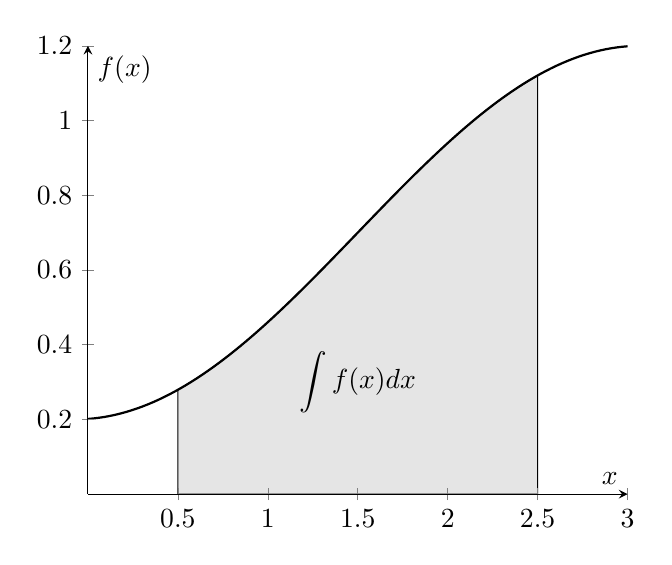
\begin{tikzpicture}
	\begin{axis}[
	axis lines = middle,
	xlabel = \(x\),
	ylabel = {\(f(x)\)},
	ymin=0, ymax=1.2,
	xmin=0, xmax=3,
	area style,
	]
	\addplot[
	fill=gray!20,
	domain=0.5:2.5,
	samples=100,
	] {0.5*sin(deg(x-1.5))+0.7} \closedcycle;
	\addplot[
	domain=0:3,
	samples=100,
	thick,
	] {0.5*sin(deg(x-1.5))+0.7};
	\node at (axis cs:1.5,0.3) {\(\displaystyle\displaystyle\int f(x)dx\)};
	\end{axis}
	\end{tikzpicture}
	\caption{\( f \) de signe constant}
	\label{fig5.1}
\end{figure}

\begin{figure}[H]
	\centering
	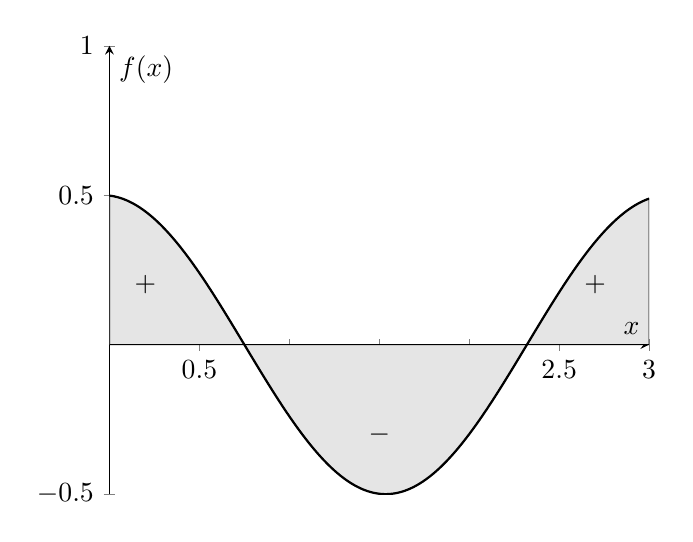
\begin{tikzpicture}
	\begin{axis}[
	axis lines = middle,
	xlabel = \(x\),
	ylabel = {\(f(x)\)},
	ymin=-0.5, ymax=1,
	xmin=0, xmax=3,
	]
	\addplot[
	fill=gray!20,
	domain=0:3,
	samples=1000,
	] {-0.5*sin(deg(2*x-1.5))} \closedcycle;
%	\addplot[
%	fill=gray!20,
%	domain=1.5:3,
%	samples=1000,
%	] {-0.5*sin(deg(2*x-1.5))} \closedcycle;
	\addplot[
	domain=0:3,
	samples=1000,
	thick,
	] {(-0.5*sin(deg(2*x-1.5))};
	\node at (axis cs:0.2,0.2) {$ + $};
	\node at (axis cs:1.5,-0.3) {$ - $};
	\node at (axis cs:2.7,0.2) {$ + $};
	\end{axis}
	\end{tikzpicture}
	\caption{\( f \) change de signe}
	\label{fig5.2}
\end{figure}

\section{Principe du calcul approché de l'intégrale}
L'interprétation géométrique de l'intégrale suggère de décomposer la surface sous le graphe de la fonction en éléments d'aires simples (rectangles, triangles, trapèzes ...).

L'idée est donc de subdiviser le segment \([a,b]\) en plusieurs sous-segments \([a_i,a_{i+1}]\) où \((i = 0,...,n-1, a_0 = a, a_n = b)\).

\[
\displaystyle\int_a^b f(t)dt = \displaystyle\sum_{i=0}^{n-1} \displaystyle\int_{a_i}^{a_{i+1}} f(t)dt
\]

on est donc ramené à évaluer \(\displaystyle\int_{a_i}^{a_{i+1}} f(t)dt\) sur un petit segment \([a_i,a_{i+1}]\) où \(f\) ne varie pas trop. Ce qui nous amène à proposer la formule approximative suivante sur un petit intervalle \([a,\beta]\) de \([a,b]\):

\begin{equation}\label{equa5.1}
\displaystyle\int_a^\beta f(t)dt = I_{a,\beta}(f) + R_{a,\beta}(f).
\end{equation}

\(I_{a,\beta}(f)\) est l'approximation proposée, \(R_{a,\beta}(f)\) est un reste : "l'erreur de la méthode" \eqref{equa5.1} est dite formule simple ou élémentaire. La formule \eqref{equa5.1} appliquée sur chaque segment \([a_i,a_{i+1}]\) nous donne la formule approximative Composée :

\[
\displaystyle\int_a^b f(t)dt = \displaystyle\sum_{i=0}^{n-1} I_{a_i,a_{i+1}}(f) + \displaystyle\sum_{i=0}^{n-1} R_{a_i,a_{i+1}}(f).
\]

Dans tout ce qui suit nous considérons la subdivision suivante :

\[
a_0 = a, a_i = a + ih, a_n = b \text{ avec } h = \frac{b-a}{n}, i = 0,...,n.
\]

cette subdivision est appelée la subdivision régulière de pas \(h\).
\begin{figure}[H]
	\centering
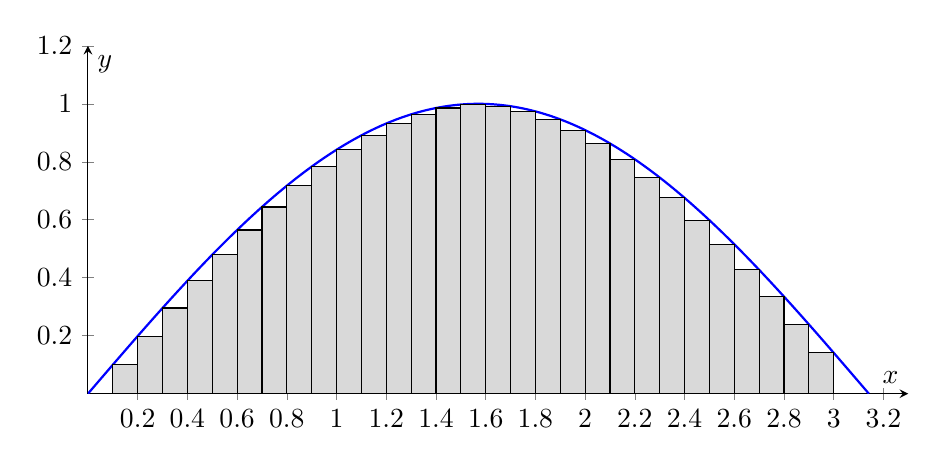
\begin{tikzpicture}
\begin{axis}[
axis lines=middle,
xlabel={$x$}, ylabel={$y$},
xmin=0, xmax=3.3,
ymin=0, ymax=1.2,
width=12cm, height=6cm,
xtick={0,0.2,...,3.2},
ytick={0,0.2,...,1.2}
]

% Courbe y = sin(x)
\addplot [
domain=0:pi,
samples=1000,
thick,
blue
] {sin(deg(x))};

% Rectangles méthode des rectangles à droite
\addplot [
ybar interval,
fill=gray!30,
draw=black,
bar width=0.1
]
plot coordinates {
	(0.1,{sin(deg(0.1))})
	(0.2,{sin(deg(0.2))})
	(0.3,{sin(deg(0.3))})
	(0.4,{sin(deg(0.4))})
	(0.5,{sin(deg(0.5))})
	(0.6,{sin(deg(0.6))})
	(0.7,{sin(deg(0.7))})
	(0.8,{sin(deg(0.8))})
	(0.9,{sin(deg(0.9))})
	(1.0,{sin(deg(1.0))})
	(1.1,{sin(deg(1.1))})
	(1.2,{sin(deg(1.2))})
	(1.3,{sin(deg(1.3))})
	(1.4,{sin(deg(1.4))})
	(1.5,{sin(deg(1.5))})
	(1.6,{sin(deg(1.7))})
	(1.7,{sin(deg(1.8))})
	(1.8,{sin(deg(1.9))})
	(1.9,{sin(deg(2.0))})
	(2.0,{sin(deg(2.1))})
	(2.1,{sin(deg(2.2))})
	(2.2,{sin(deg(2.3))})
	(2.3,{sin(deg(2.4))})
	(2.4,{sin(deg(2.5))})
	(2.5,{sin(deg(2.6))})
	(2.6,{sin(deg(2.7))})
	(2.7,{sin(deg(2.8))})
	(2.8,{sin(deg(2.9))})
	(2.9,{sin(deg(3.0))})
	(3.0,{sin(deg(0.05))})
};

\end{axis}
\end{tikzpicture}
	\caption{Subdivision de \([a, b]\) et approximation de \(\displaystyle \displaystyle\int_a^b f(x) dx\) par la somme des surfaces hachurées}
\end{figure}

\section{Formule des rectangles (avec point milieu)}
\subsection{Formule élémentaire}
On remplace le graphe de la fonction \(f\) entre \([a, \beta]\) par une droite \(y = f(\gamma)\), où \(\gamma = \frac{\alpha + \beta}{2}\) est le point milieu de \([a, \beta]\). (voir figure \ref{recM})

\begin{figure}[H]
	\centering
	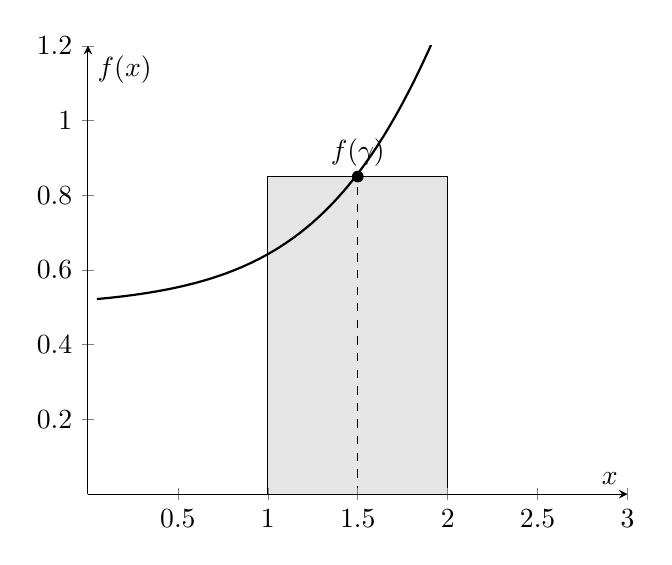
\begin{tikzpicture}
	\begin{axis}[
	axis lines = middle,
	xlabel = \(x\),
	ylabel = {\(f(x)\)},
	ymin=0, ymax=1.2,
	xmin=0, xmax=3,
	area style,
	]
	
	
	% Rectangle
	\draw[fill=gray!20] (axis cs:1,0) rectangle (axis cs:2,0.85);
	\draw[dashed] (axis cs:1.5,0) -- (axis cs:1.5,0.85);
	
	% Points
	\node[circle,fill,inner sep=1.5pt] at (axis cs:1.5,0.85) {};
	\node[above] at (axis cs:1.5,0.85) {\(f(\gamma)\)};
	
	% Labels
	\node[below] at (axis cs:1,0) {\(\alpha\)};
	\node[below] at (axis cs:2,0) {\(\beta\)};
	\node[below] at (axis cs:1.5,0) {\(\gamma\)};
	
	% Function
	\addplot[
	domain=0.05:4.5,
	samples=1000,
	thick,
	] {2+1.5*tanh(x-2.5)};
	\end{axis}
	\end{tikzpicture}
	\caption{Méthode des rectangles avec point milieu.}
	\label{recM}
\end{figure}

\[
\displaystyle\int_a^\beta f(t) dt \approx h f(\gamma) + R_{\alpha, \beta}(f), \quad h = \beta - \alpha.
\]

\subsection{Estimation du reste \(R_{\alpha, \beta}\)}
Supposons que \(f\) a une dérivée seconde continue (\(F\) aura donc une dérivée tierce continue). La formule de Taylor à l'ordre 3 entre \(\gamma\) et \(\beta\) appliquée à \(F\) :

\begin{multline}\label{eqa2.5.1}
F(\beta) - F(\gamma) = (\beta - \gamma) F'(\gamma) + \frac{(\beta - \gamma)^2}{2} F''(\gamma) + \frac{(\beta - \gamma)^3}{3!} F'''(\epsilon)\\
= \frac{h}{2} f(\gamma) + \frac{h^2}{8} f'(\gamma) + \frac{h^3}{48} f''(\epsilon), \quad \epsilon \in [\gamma, \beta] 
\end{multline}

Formule de Taylor entre \(\alpha\) et \(\gamma\) :

\begin{equation}\label{eqa2.5.2}
F(\alpha) - F(\gamma) = -\frac{h}{2} f(\gamma) + \frac{h^2}{8} f'(\gamma) - \frac{h^3}{48} f''(\eta), \quad \eta \in [\alpha, \gamma] 
\end{equation}

En retranchant \eqref{eqa2.5.1} de \eqref{eqa2.5.2} on obtient la relation :

\[
F(\beta) - F(\alpha) = hf(\gamma) + \frac{h^3}{24} \frac{f''(\eta) + f''(\epsilon)}{2}
\]

\( f'' \) est une fonction continue, d'après le théorème des valeurs intermédiaires il existe \( \theta \in ]\eta,\epsilon[ \) telle que 

\[
\frac{1}{2}(f''(\eta) + f''(\epsilon)) = f''(\theta)
\]

La formule élémentaire devient donc :

\[
\displaystyle\int_{\alpha}^{\beta} f(t)dt = hf(\gamma) + \frac{h^3}{24} f''(\theta), \quad \alpha < \theta < \beta.
\]

\subsection{Formule composée}
Supposons que \( f : [a,b] \rightarrow \mathbb{R} \) a une dérivée seconde \( f'' \) continue, considérons la subdivision \((a_i)_i=0,1,...,n\) de pas \( h = \frac{b-a}{n} \), sur chaque intervalle \([a_i,a_{i+1}]\) on a la formule élémentaire :

\[
\displaystyle\int_{a_i}^{a_{i+1}} f(t)dt = hf(\gamma_i) + \frac{h^3}{24} f''(\theta_i), \quad a_i < \theta_i < a_{i+1} \text{ avec } \gamma_i = \frac{a_i + a_{i+1}}{2}.
\]

d'ou la formule composée suivante :

\[
\displaystyle\int_a^b f(t)dt = h \displaystyle\sum_{i=0}^{n-1} f(\gamma_i) + n \frac{h^3}{24} \displaystyle\sum_{i=0}^{n-1} \frac{1}{n} f''(\theta_i).
\]

Or, \( f'' \) est continue, d'après le théorème des valeurs intermédiaires, il existe \( \theta \in [a,b] \) tel que :

\[
\frac{1}{n} \displaystyle\sum_{i=0}^{n-1} f''(\theta_i) = f''(\theta)
\]

en tenant compte du fait que \( nh = (b-a) \), on obtient comme formule composée :

\[
\displaystyle\int_a^b f(t)dt = = \underbrace{h \sum_{i=0}^{n-1} f\left(\dfrac{a_i+a_{i+1}}{2}\right)}_{Q_n(f)} + \underbrace{\dfrac{h^2}{24}(b-a)f''(\theta)}_{R_n(f)}.
\]

\begin{figure}[H]
	\centering
	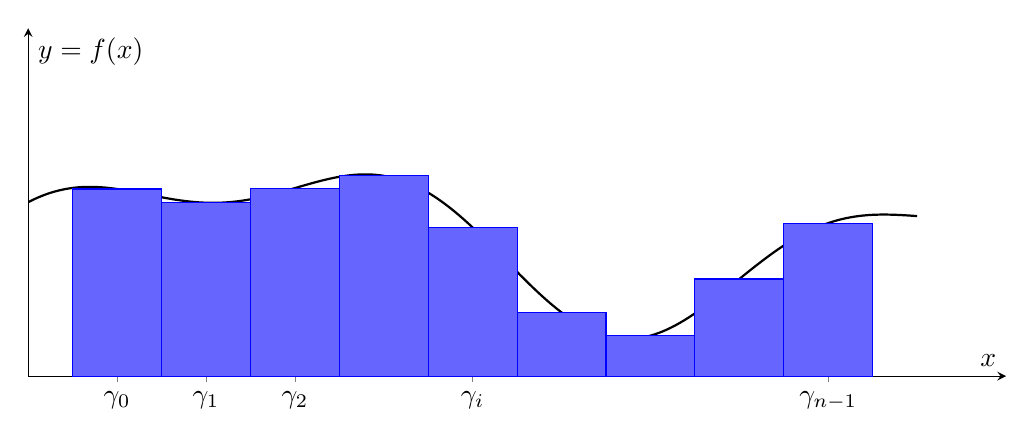
\begin{tikzpicture}
	\begin{axis}[
	axis lines=middle,
	xlabel={$x$}, ylabel={$y=f(x)$},
	xmin=0, xmax=11,
	ymin=0, ymax=5,
	xtick={1,2,3,5,9},
	xticklabels={$ \gamma_0$, $\gamma_1$, $\gamma_2$, $\gamma_i$, $\gamma_{n-1}$},
	ytick=\empty,
	width=14cm, height=6cm,
	enlargelimits=false
	]
	
	% Courbe f(x) (exemple sinusoïde modifiée)
	\addplot [
	domain=0:10,
	samples=200,
	thick
	] {2+sin(deg(x/1.5)) + 0.5*cos(deg(x/0.7))};
	
	% Rectangles (méthode de Riemann généralisée)
	\addplot [
	ybar,
	bar width=1,
	fill=blue!60,
	draw=blue
	]
	coordinates {
		(1,{2+sin(deg(1/1.5))+0.5*cos(deg(1/0.7))})
		(2,{2+sin(deg(2/1.5))+0.5*cos(deg(2/0.7))})
		(3,{2+sin(deg(3/1.5))+0.5*cos(deg(3/0.7))})
		(4,{2+sin(deg(4/1.5))+0.5*cos(deg(4/0.7))})
		(5,{2+sin(deg(5/1.5))+0.5*cos(deg(5/0.7))})
		(6,{2+sin(deg(6/1.5))+0.5*cos(deg(6/0.7))})
		(7,{2+sin(deg(7/1.5))+0.5*cos(deg(7/0.7))})
		(8,{2+sin(deg(8/1.5))+0.5*cos(deg(8/0.7))})
		(9,{2+sin(deg(9/1.5))+0.5*cos(deg(9/0.7))})
	};
	
	% Labels pour a et b
	\node at (axis cs:0,0) [below] {$a$};
	\node at (axis cs:10,0) [below] {$b$};
	
	\end{axis}
	\end{tikzpicture}
	\caption{Méthode des rectangles avec point milieu.}
\end{figure}

\subsection{Propriétés}
\begin{enumerate}
	\item Si \( f'' = 0 \) sur \([a, b]\) c-à-d \( f \) est un polynôme de degré un ou moins, il n'y a pas d'erreur de méthode.
	\item Si \( f'' \geq 0 \) l'approximation de \( \displaystyle\int_a^b f(t)dt \) fournie par \( Q_n(f) \) est par excès.
	\item La méthode est convergente, en effet si \( M \) est un majorant de \( |f''| \) sur \([a, b]\) on a :
	\[
	|R_n(f)| \leq \frac{h^2}{24}(b-a)M \text{ proportionnelle } \hat{a} \frac{1}{n^2} \to 0.
	\]
\end{enumerate}

\subsection{Estimation de l'erreur}
- si \( f'' \leq M \) sur \([a, b]\) on a une estimation à priori de l'erreur \( \frac{h^2}{24}(b-a)M \)

- Pour limiter le nombre d'évaluations de \( f \), on peut se limiter au cas où \( n \) est une puissance de 3 ( \( n : 1, 3, 9, 27, ... \) ). \( |Q_n - Q_{3^n}| \) fournit en général une estimation de l'erreur.

\subsection{Exemple 5.1}
\[
Log(2) = \displaystyle\int_1^2 \frac{1}{t} dt \approx 0.6931471806
\]

\[
f(x) = \frac{1}{x}, \quad f'(x) = -\frac{1}{x^2}, \quad f''(x) = \frac{2}{x^3}, \quad |f''(x)| \leq 2 = M, \quad \forall x \geq 1
\]

- Si \( n = 1 \) on \( a : h = \frac{2-1}{1} = 1, a_0 = 1, a_1 = 2 = 1 + 1h \) donc \( \gamma_0 = \frac{a_0+a_1}{2} = \frac{3}{2} \) d'où

\[
Q_1 = h \displaystyle\sum_{i=0}^{1-1} f(\gamma_i) = hf(\gamma_0) = f\left(\frac{3}{2}\right) = \frac{2}{3} = 0.66666666.
\]

- Si \( n = 3 \) on \( a : h = \frac{2-1}{3} = \frac{1}{3}, a_0 = 1, a_1 = 1 + 1\frac{1}{3} = \frac{4}{3}, a_2 = 1 + 2\frac{1}{3} = \frac{5}{3} \) et \( a_3 = 1 + 3\frac{1}{3} = 2 \) donc :

\[
\gamma_0 = \frac{a_0+a_1}{2} = \frac{7}{6}, \quad \gamma_1 = \frac{a_1+a_2}{2} = \frac{9}{6}, \quad \gamma_2 = \frac{a_2+a_3}{2} = \frac{11}{6} \, d'où
\]

\[
Q_3 = h \displaystyle\sum_{i=0}^{3-1} f(\gamma_i) = h(f(\gamma_0) + f(\gamma_1) + f(\gamma_2)) = \frac{1}{3} \left( \frac{6}{7} + \frac{6}{9} + \frac{6}{11} \right) = \frac{478}{693} = 0.68975468
\]

- Si \( n = 9 \) on \( a : h = \frac{1}{9}, a_0 = 1, a_1 = 1 + 1\frac{1}{9} = \frac{10}{9}, a_2 = 1 + 2\frac{1}{9} = \frac{11}{9}, a_i = 1 + i\frac{1}{9} \) et \( a_9 = 2 \) donc :

\[
\gamma_0 = \frac{a_0+a_1}{2} = \frac{19}{18}, \quad \gamma_1 = \frac{a_1+a_2}{2} = \frac{21}{18}, \quad \gamma_i = \frac{a_i+a_{i+1}}{2} = \frac{19+2i}{18} \, d'où
\]

\begin{align*}
Q_9 &= h \displaystyle\sum_{i=0}^{9-1} f(\gamma_i)\\
&= h(f(\gamma_0) + f(\gamma_1) + ... + f(\gamma_8))\\
&= \frac{1}{9} \left( \frac{18}{19} + \frac{18}{21} + ... + \frac{18}{19+2i} + ... + \frac{18}{35} \right)\\
&= \frac{14145553414}{20419054425} = 0.69276237
\end{align*}

\begin{table}[H]
	\centering
	\begin{tabular}{ccccc}
		\(n\) & \(Q_n\) & \((b-a)\frac{h^2M}{24}\) & \(|Q_n - Q_{3^n}|\) & erreur exacte \\
		\hline
		1 & 0.66666667 & \(8.3\times10^{-2}\) & - & \(-2.7\times10^{-2}\) \\
		3 & 0.68975468 & \(4.6\times10^{-3}\) & \(2.3\times10^{-2}\) & \(-3.4\times10^{-3}\) \\
		9 & 0.69276237 & \(5.2\times10^{-3}\) & \(3.0\times10^{-3}\) & \(-3.9\times10^{-4}\) \\
	\end{tabular}
\end{table}

\section{La méthode des trapèzes}
Cette méthode consiste à remplacer la courbe de la fonction \( f \) entre \( \alpha \) et \( \beta \) par une droite passant par les deux points \( (\alpha, f(\alpha)) \) et \( (\beta, f(\beta)) \). Ceci est schématisé dans la figure suivante :

\begin{figure}[H]
	\centering
	\begin{tikzpicture}
	\begin{axis}[
	axis lines=middle,
	xlabel={$x$}, ylabel={$y=f(x)$},
	xmin=-1, xmax=5,
	ymin=0, ymax=4,
	xtick={1,4},
	xticklabels={$\alpha$, $\beta$},
	ytick=\empty,
	width=8cm, height=6cm
	]
	
	% Définition de la fonction f(x)
	\addplot [
	domain=0:5,
	samples=200,
	thick
	] {ln(x+1)+1};
	
	% Polygone du trapèze
	\addplot [
	fill=red!60,
	fill opacity=0.6,
	pattern=north east lines,
	pattern color=red
	]
	coordinates {(1,0) (1,{ln(2)+1}) (4,{ln(5)+1}) (4,0)} -- cycle;
	
	% Ligne horizontale f(α)
	\draw[dashed] (axis cs:0,{ln(2)+1}) -- (axis cs:1,{ln(2)+1});
	\node[left] at (axis cs:0,{ln(2)+1}) {$f(\alpha)$};
	
	% Ligne horizontale f(β)
	\draw[dashed] (axis cs:0,{ln(5)+1}) -- (axis cs:4,{ln(5)+1});
	\node[left] at (axis cs:0,{ln(5)+1}) {$f(\beta)$};
	\end{axis}
	\end{tikzpicture}
	\caption{Méthode du trapèze.}
\end{figure}

\[
\displaystyle\int_{\alpha}^{\beta} f(t)dt = \frac{h}{2}(f(\alpha) + f(\beta)) + R_{\alpha, \beta}(f).
\]

Pour exprimer le reste \( R_{\alpha, \beta}(f) \), on suppose que \( f \) a une dérivée seconde \( f'' \) continue sur \( [\alpha, \beta] \) et introduisons la fonction auxiliaire \( \varphi(x) \) définie par :

\[
\varphi(x) = F(\gamma + x) - F(\gamma - x) - x(f(\gamma + x) + f(\gamma - x)) - kx^3, \quad \gamma = \frac{\alpha + \beta}{2}. \tag{5.4}
\]

k est une constante choisie telle que \( \varphi(\frac{h}{2}) = 0 \). En exigeant cela on obtient pour k l'expression suivante :

\[
k = \frac{F(\beta) - F(\alpha) - \frac{h}{2}(f(\beta) + f(\alpha))}{(h/2)^3}
\]

\( \varphi(0) = \varphi(h/2) = 0 \), d'après le théorème de Rolle il existe \( e \in ]0, h/2[ \) telle que \( \varphi'(e) = 0 \), or

\[
\varphi'(x) = -x(f'(\gamma + x) - f'(\gamma - x)) - 3kx^2
\]

Le théorème des accroissements finis appliqué à \( f' \) sur l'intervalle \( |\gamma - e, \gamma + e| \) implique qu'il existe \( \eta \in ]\gamma - e, \gamma + e| \) telle que

\[
f'(\gamma + e) - f'(\gamma - e) = 2ef''(\eta)
\]

comme \( \varphi'(e) = 0 \) on obtient \( k = -\frac{2}{3}f''(\eta) \) et comme \( \varphi(\frac{h}{2}) = 0 = F(\beta) - F(\alpha) - \frac{h}{2}(f(\beta) + f(\alpha)) + \frac{2}{3}f''(\eta)(\frac{h}{2})^3 \), on en déduit :

\[
\displaystyle\int_{\alpha}^{\beta} f(t)dt = \frac{h}{2}(f(\beta) + f(\alpha)) - \frac{h^3}{12}f''(\eta), \quad \alpha < \eta < \beta
\]

c'est la formule élémentaire pour la méthode des trapèzes.

\subsection{Formule composée}
On suppose que \( f : [a, b] \) vers \( R \) a une dérivée seconde continue \( f'' \). On considère la subdivision régulière de pas \( h \) de \([a, b]: a_0 = a < a_1 < a_2 < ... < a_n = b \), sur chaque \([a_i, a_{i+1}]\) on a par application de la formule élémentaire :

\[
\displaystyle\int_{a_i}^{a_{i+1}} f(t)dt = \frac{h}{2} (f(a_i) + f(a_{i+1})) - \frac{h^3}{12} f''(\epsilon_i), \quad a_i < \epsilon_i < a_{i+1}
\]

sur l'intervalle \([a, b]\) on a donc :

\[
\displaystyle\int_a^b f(t)dt = \frac{h}{2} \displaystyle\sum_{i=0}^{n-1} (f(a_i) + f(a_{i+1})) - \frac{h^3}{12} \displaystyle\sum_{i=0}^{n-1} f''(\epsilon_i)
\]

\[
= h \left( \frac{f(a)}{2} + \displaystyle\sum_{i=1}^{n-1} f(a_i) + \frac{f(b)}{2} \right) - \frac{h^2}{12} (b-a) f''(\theta)
\]

\[
T_n(f) \quad R_n(f)
\]

\( T_n(f) \) est la valeur approchée de \( \displaystyle\int_a^b f(t)dt \). \( R_n(f) \) est l'erreur de la méthode lorsqu'on approche \( \displaystyle\int_a^b f(t)dt \) par \( T_n(f) \). La figure suivante permet de schématiser cette méthode d'approximation :

\begin{figure}[H]
	\centering
	\begin{tikzpicture}[scale=1]
	% Définition de la fonction (garantie positive)
	\def\func#1{2.3 + 0.2*sin(100*(#1-0.8)) + 0.6*cos(150*(#1-2))}
	
	% Axes
	\draw[->] (-0.2,0) -- (6.5,0) node[right] {$x$};
	\draw[->] (0,-0.2) -- (0,3.5) node[above] {$y=f(x)$};
	
	% Points de subdivision
	\def\xa{0.8}    % a0=a
	\def\xb{1.5}    % a1  
	\def\xc{2.2}    % a2
	\def\xd{3.4}    % ai
	\def\xe{4.7}    % an-1
	\def\xf{5.5}    % an=b
	
	% Trapèze 1
	\fill[red!70] (\xa,0) -- (\xa,{\func{\xa}}) -- (\xb,{\func{\xb}}) -- (\xb,0) -- cycle;
	\draw[pattern=north east lines, pattern color=black!50] (\xa,0) -- (\xa,{\func{\xa}}) -- (\xb,{\func{\xb}}) -- (\xb,0) -- cycle;
	
	% Trapèze 2
	\fill[red!70] (\xb,0) -- (\xb,{\func{\xb}}) -- (\xc,{\func{\xc}}) -- (\xc,0) -- cycle;
	\draw[pattern=north east lines, pattern color=black!50] (\xb,0) -- (\xb,{\func{\xb}}) -- (\xc,{\func{\xc}}) -- (\xc,0) -- cycle;
	
	% Trapèzes intermédiaires
	\pgfmathsetmacro{\step}{0.3}
	\foreach \i in {2.2, 2.5, 2.8, 3.1} {
		\pgfmathsetmacro{\inext}{\i + \step}
		\fill[red!70] (\i,0) -- (\i,{\func{\i}}) -- (\inext,{\func{\inext}}) -- (\inext,0) -- cycle;
		\draw[pattern=north east lines, pattern color=black!50] (\i,0) -- (\i,{\func{\i}}) -- (\inext,{\func{\inext}}) -- (\inext,0) -- cycle;
	}
	
	% Trapèze ai
	\fill[red!70] (\xd,0) -- (\xd,{\func{\xd}}) -- (3.8,{\func{3.8}}) -- (3.8,0) -- cycle;
	\draw[pattern=north east lines, pattern color=black!50] (\xd,0) -- (\xd,{\func{\xd}}) -- (3.8,{\func{3.8}}) -- (3.8,0) -- cycle;
	
	% Trapèzes vers la fin
	\foreach \i in {3.8, 4.1, 4.4} {
		\pgfmathsetmacro{\inext}{\i + \step}
		\fill[red!70] (\i,0) -- (\i,{\func{\i}}) -- (\inext,{\func{\inext}}) -- (\inext,0) -- cycle;
		\draw[pattern=north east lines, pattern color=black!50] (\i,0) -- (\i,{\func{\i}}) -- (\inext,{\func{\inext}}) -- (\inext,0) -- cycle;
	}
	
	% Trapèze an-1
	\fill[red!70] (\xe,0) -- (\xe,{\func{\xe}}) -- (\xf,{\func{\xf}}) -- (\xf,0) -- cycle;
	\draw[pattern=north east lines, pattern color=black!50] (\xe,0) -- (\xe,{\func{\xe}}) -- (\xf,{\func{\xf}}) -- (\xf,0) -- cycle;
	
	% Courbe de la fonction (par-dessus les trapèzes)
	\draw[thick, black] plot[domain=0.4:6.0, samples=400] 
	(\x, {\func{\x}});
	
	% Lignes verticales pour les subdivisions principales
	\foreach \x in {\xa, \xb, \xc, \xd, \xe, \xf} {
		\draw[thin, black] (\x,0) -- (\x,-0.1);
	}
	
	% Labels des points
	\node[below] at (\xa,-0.2) {$a_0=a$};
	\node[below] at (\xb,-0.2) {$a_1$};
	\node[below] at (\xc,-0.2) {$a_2$};
	\node[below] at (\xd,-0.2) {$a_i$};
	\node[below] at (\xe,-0.2) {$a_{n-1}$};
	\node[below] at (\xf,-0.2) {$a_n=b$};
	
	\end{tikzpicture}
	\caption{Méthode des trapèzes}
\end{figure}

\subsection{Propriétés}
\begin{itemize}
	\item si \( f'' = 0 \) alors \( R_n(f) = 0 \).
	\item si \( f'' > 0 \) l'approximation fournit par \( T_n(f) \) est par défaut.
	\item si \( f'' \geq 0 \) et garde le même signe sur un intervalle \([a, b]\) on peut encadrer l'intégrale \( \displaystyle\int_a^b f(t)dt \) par :
	\[
	Q_n(f) \leq \displaystyle\int_a^b f(t)dt \leq T_n(f).
	\]
	\item la méthode est convergente : la convergence est en \( \frac{1}{n^2} \).
\end{itemize}

\subsection{Estimation de l'erreur}
- Si \( f'' \) est Majorée par \( M \) on a : \( |R_n(f)| \leq \frac{(b-a)h^2M}{12} \).
- Pour limiter le nombre d'évaluations de \( f \), on peut se limiter au cas où \( n \) est une puissance de 2, alors dans ce cas \( |T_{2^n} - T_n| \) fournit une estimation de l'erreur ainsi qu'un test d'arrêt des itérations.

\subsection{Exemple}
\[
Log(2) = \displaystyle\int_{1}^{2} \frac{1}{t} dt \approx 0.6931471806
\]

\begin{table}[H]
	\centering
	\begin{tabular}{ccccc}
		\(n\) & \(T_n\) & \(\frac{(b-a)h^2M}{12}\) & \(|T_{2^n} - T_n|\) & erreur exacte \\
		\hline
		1 & 0.75 & \(8.3\times10^{-2}\) & - & \(5.7\times10^{-2}\) \\
		2 & 0.7083333 & \(2.1\times10^{-2}\) & \(4.7\times10^{-2}\) & \(1.5\times10^{-2}\) \\
		4 & 0.6970238 & \(5.2\times10^{-3}\) & \(1.1\times10^{-2}\) & \(3.4\times10^{-3}\) \\
		8 & 0.69412183 & \(1.3\times10^{-3}\) & \(2.9\times10^{-3}\) & \(9.8\times10^{-4}\) \\
	\end{tabular}
\end{table}

\section{Méthode de Simpson}
\subsection{Formule élémentaire}
Pour établir la formule élémentaire des rectangles et des trapèzes, on a en fait interpolé la fonction \( f \) :
- par une droite horizontale ( un polynôme de degré 0) dans la méthode des rectangles avec point milieu.
- par une droite ( un polynôme de degré 1 ) dans la méthode des trapèzes.

On peut espérer améliorer la précision en approchant le graphe de \( f \) par l'arc de parabole d'axe vertical, passant par les points \( A(\alpha, f(\alpha)) \), \( B(\beta, f(\beta)) \) et \( C(\gamma, f(\gamma)) \) (avec \( \gamma = \frac{\alpha + \beta}{2} \)). Ce qui revient à interpoler \( f \) en ces points par un polynôme de degré 2.

On montre facilement que le polynôme de degré 2 qui passe par \( A \), \( B \) et \( C \) est de la forme :

\[
P(x) = \frac{(x-\gamma)(x-\beta)}{(\alpha-\gamma)(\alpha-\beta)}f(\alpha) + \frac{(x-\alpha)(x-\beta)}{(\gamma-\alpha)(\gamma-\beta)}f(\gamma) + \frac{(x-\alpha)(x-\gamma)}{(\beta-\alpha)(\beta-\gamma)}f(\beta)
\]

\[
= \frac{2}{h^2}[(x-\gamma)(x-\beta)f(\alpha)-2(x-\alpha)(x-\beta)f(\gamma)+(x-\alpha)(x-\gamma)f(\beta)]
\]

On a donc \( \displaystyle\int_{\alpha}^{\beta} P(x)dx = \frac{h}{6}(f(\alpha)+4f(\gamma)+f(\beta)) \) on propose donc la formule élémentaire suivante :

\[
\displaystyle\int_{\alpha}^{\beta} f(t)dt = \frac{h}{6}(f(\alpha)+4f(\gamma)+f(\beta))+R_{\alpha,\beta}
\]

pour exprimer le reste, en est amené à supposer que \( f \) a une dérivé quatrième \( f^4 \) continue : considérons la fonction auxiliaire : \( \varphi : [0, \frac{h}{2}] \rightarrow R \) définie par

\[
\varphi(x) = F(\gamma+x)-F(\gamma-x) - \frac{x}{3}(f(\gamma+x)+f(\gamma-x)+4f(\gamma))+kx^5
\]

\( k \) est une constante choisie telle que : \( \varphi(\frac{h}{2}) = 0 \).

\( \varphi(0) = \varphi(\frac{h}{2}) = 0 \), d'après le théorème de Rolle, il existe \( e_1 \in [0, \frac{h}{2}] \) telle que \( \varphi'(e_1) = 0 \). D'après l'expression de \( \varphi'(x) \) donnée ci-dessous

\[
\varphi'(x) = \frac{2}{3}(f(\gamma+x)+f(\gamma-x)) - \frac{4}{3}f(\gamma) - \frac{x}{3}(f'(x+\gamma)-f'(\gamma-x))+5kx^4
\]

on conclut que \( \varphi'(0) = 0 \), et comme \( \varphi'(e_1) = 0 \) on en déduit du théorème de Rolle qu'il existe \( e_2 \in [0, e_1] \) telle que \( \varphi''(e_2) = 0 \)

\[
\phi''(x) = \frac{1}{3}(f'(y+x)-f'(y-x))-\frac{x}{3}(f''(x+y)+f''(y-x))+20kx^3
\]

\begin{figure}[H]
	\centering
	\begin{tikzpicture}
	\begin{axis}[
	axis lines=middle,
	xlabel={$x$}, 
	ylabel={$y=f(x)$},
	xmin=-1, xmax=5,
	ymin=0, ymax=4,
	xtick={1,2.5,4},
	xticklabels={$\alpha$,$\gamma$, $\beta$},
	ytick=\empty,
	width=8cm, height=6cm,
	xlabel style={anchor=west},
	ylabel style={anchor=south}
	]
	
	% Définition de la fonction f(x) = ln(x-0.5) + 1
	\addplot [
	domain=0.6:4.5,
	samples=200,
	thick,
	black
	] {ln(x-0.5)+1};
	
	% Zone du trapèze avec deux couleurs
	% Première partie (α à γ) en bleu
	\addplot [
	fill=cyan!40,
	fill opacity=0.7,
	pattern=north east lines,
	pattern color=cyan!80,
	draw=none
	]
	coordinates {(1,0) (1,{ln(0.5)+1}) (2.5,{ln(2)+1}) (2.5,0)} -- cycle;
	
	% Deuxième partie (γ à β) en rouge
	\addplot [
	fill=red!40,
	fill opacity=0.7,
	pattern=north east lines,
	pattern color=red!80,
	draw=none
	]
	coordinates {(2.5,0) (2.5,{ln(2)+1}) (4,{ln(3.5)+1}) (4,0)} -- cycle;
	
	% Contour du trapèze
	\addplot [
	thick,
	black,
	no markers
	]
	coordinates {(1,{ln(0.5)+1}) (2.5,{ln(2)+1}) (4,{ln(3.5)+1})};
	
	% Lignes verticales
	\draw[thick] (axis cs:1,0) -- (axis cs:1,{ln(0.5)+1});
	\draw[thick] (axis cs:2.5,0) -- (axis cs:2.5,{ln(2)+1});
	\draw[thick] (axis cs:4,0) -- (axis cs:4,{ln(3.5)+1});
	
	% Lignes horizontales pointillées
	\draw[dashed, gray] (axis cs:0,{ln(0.5)+1}) -- (axis cs:1,{ln(0.5)+1});
	\node[left] at (axis cs:0,{ln(0.5)+1}) {$f(\alpha)$};
	
	\draw[dashed, gray] (axis cs:0,{ln(2)+1}) -- (axis cs:2.5,{ln(2)+1});
	\node[left] at (axis cs:0,{ln(2)+1}) {$f(\gamma)$};
	
	\draw[dashed, gray] (axis cs:0,{ln(3.5)+1}) -- (axis cs:4,{ln(3.5)+1});
	\node[left] at (axis cs:0,{ln(3.5)+1}) {$f(\beta)$};
	
	\end{axis}
	\end{tikzpicture}
	\caption{Méthode de Simpson}
\end{figure}

\[
\phi''(\epsilon_2) = 0, \quad \phi''(0) = 0; \text{ par application du théorème de Rolle de nouveau, il existe } \epsilon_3 \in [0,\epsilon_2]
\]
telle que \(\phi^{(3)}(\epsilon_3) = 0\). Le même procédé appliqué à \(\phi^{(3)}\) donne :

\[
\phi^{(3)}(x) = -\frac{x}{3}(f^{(3)}(x+y)-f^{(3)}(y-x))+60kx^2
\]

\[
\phi^{(3)}(\epsilon_3) = 0 \text{ implique } \frac{\epsilon_3}{3}(f^{(3)}(\epsilon_3+y)-f^{(3)}(y-\epsilon_3))=60k\epsilon_3^2.
\]
Le théorème des accroissements assure l'existence de \(\eta \in ]\gamma - \epsilon_3, \gamma + \epsilon_3[\) tel que

\[
f^{(3)}(\epsilon_3+\gamma)-f^{(3)}(\gamma-\epsilon_3)=2\epsilon_3f^{(4)}(\eta)
\]

On a donc finalement :

\[
k = \frac{1}{90}f^{(4)}(\eta)
\]

avec cette valeur de \(k\) mise dans l'expression de la fonction auxiliaire et en demandant que \(\phi(\frac{h}{2}) = 0\) on en déduit :

\[
\displaystyle\int_a^\beta f(t)dt = F(\beta)-F(\alpha) = \frac{h}{6}(f(\beta)+f(\alpha)+4f(\gamma))-\frac{h^5}{2880}f^{(4)}(\eta)
\]

ceci est la formule élémentaire pour la méthode de Simpson.

\subsection{Formule composée}
On suppose que \(f: [a,b]\) vers \(R\) a une dérivée quatrième \(f^4\) continue. On considère une subdivision régulière de pas \(h = \frac{b-a}{n}\) de \([a,b]: a_0 = a < a_1 < a_2 < ... < a_n = b\) sur chaque intervalle \([a_i,a_{i+1}]\) on a :

\[
\displaystyle\int_{a_i}^{a_{i+1}} f(t)dt = F(a_{i+1})-F(a_i) = \frac{h}{6}(f(a_i)+f(a_{i+1})+4f\left(\frac{a_i+a_{i+1}}{2}\right))-\frac{h^5}{2880}f^{(4)}(\eta_i)
\]

d'où sur \([a,b]\) :

\[
\displaystyle\int_a^b f(t)dt = \frac{h}{6} \displaystyle\sum_{i=0}^{n-1} (f(a_i) + f(a_{i+1}) + 4f\left(\frac{a_i + a_{i+1}}{2}\right)) - \frac{h^5}{2880} \displaystyle\sum_{i=0}^{n-1} f^{(4)} (\eta_i)
\]

En appliquant le théorème des valeurs intermédiaire au dernier terme du membre de droite : on trouve :

\[
\displaystyle\int_a^b f(t)dt =  \underbrace{\frac{h}{6} \left(f(a) + f(b) + 2 \displaystyle\sum_{i=1}^{n-1} f(a_i) + 4 \displaystyle\sum_{i=0}^{n-1} f\left(\frac{a_i + a_{i+1}}{2}\right)\right)}_{S_n(f)}  - \underbrace{\frac{h^4}{2880} \left( b - a \right) f^{(4)} (\theta)}_{R_{n}(f)}
\]

Le reste \( R_n(f) \) représente l'erreur de méthode lorsqu'on remplace \(\displaystyle\int_a^b f(t)dt\) par la somme finie \( S_n(f) \).

\subsection{Propriétés}
\[
- R_n(f) = \displaystyle\int_a^b f(t)dt - S_n(f).
\]
\[
- \text{la méthode est convergente, sa convergence est réglée par le terme en } h^4
\]
\[
- S_n(f) = \frac{1}{3}(2Q_n(f) + T_n(f)).
\]

\subsection{Estimation de l'erreur}
En pratique il est difficile d'obtenir une majoration de la dérivée \( 4^{eme} \). Sinon, si \( M \) est un majorant de \( f^{(4)} \) on a :

\[
|R_n(f)| \leq (b - a) \frac{h^4 M}{2880}
\]

Pour limiter le nombre d'évaluations de \( f \), on peut se limiter au cas où \( n \) est une puissance de 2. Alors dans ce cas \( |S_{2^n} - S_n| \) fournit une estimation de l'erreur ainsi qu'un test d'arrêt des itérations.

\subsection{Exemple 5.3}
\[
Log(2) = \displaystyle\int_1^2 \frac{1}{t} dt \approx 0.6931471806, \, f'(x) = -\frac{1}{x^2}, \, f''(x) = \frac{2}{x^3}, \, f^3(x) = \frac{6}{x^4}, \, f^4(x) = \frac{24}{x^5}.
\]
\[\text{On remarque donc que } f^4(x) \text{ est majorée par 24.}\]

\begin{table}[H]
	\centering
	\begin{tabular}{cccccc}
		\(n\) & nombre de point & \(S_n\) & \(\frac{(b-a)h^4 M}{2880}\) & \(|S_{2^n} - S_n|\) & erreur exacte \\
		\hline
		1 & 3 & 0.69444443 & \(8.3\times10^{-3}\) & - & \(1.2\times10^{-3}\) \\
		2 & 5 & 0.69325393 & \(2.2\times10^{-4}\) & \(1.2\times10^{-3}\) & \(1.1\times10^{-4}\) \\
		4 & 9 & 0.69315450 & \(3.3\times10^{-5}\) & \(1.1\times10^{-4}\) & \(6.3\times10^{-6}\) \\
		8 & 17 & 0.69314760 & \(2.0\times10^{-6}\) & \(6.9\times10^{-6}\) & \(4.2\times10^{-7}\) \\
	\end{tabular}
\end{table}

\subsection{Conclusion}
Le tableau suivant résume les trois méthodes d'intégration numérique étudiées dans ce chapitre.

\begin{table}[H]
	\centering
	{\small
	\begin{tabular}{lll}
		Méthode & Expression de l'approximation & L'erreur de l'approximation \\
		\hline
		Quadrature & \( Q_n(f) = h \displaystyle\sum_{i=0}^{n-1} f\left(\frac{a_i + a_{i+1}}{2}\right) \) & \( R_n(f) = \frac{h^2}{24}(b - a)f''(\theta) \) \\
		Trapèze & \( T_n(f) = h \left( \frac{f(a)}{2} + \displaystyle\sum_{i=1}^{n-1} f(a_i) + \frac{f(b)}{2} \right) \) & \( R_n(f) = \frac{h^2}{12}(b - a)f''(\theta) \) \\
		Simpson & \( S_n(f) = \frac{h}{6} \left( f(a) + f(b) + 2 \displaystyle\sum_{i=1}^{n-1} f(a_i) + 4 \displaystyle\sum_{i=0}^{n-1} f\left(\frac{a_i + a_{i+1}}{2}\right) \right) \) & \( R_n(f) = \frac{h^4}{2880}(b - a)f^4(\theta) \) \\
	\end{tabular}
}
\end{table}

\section{Dérivation numérique}
Dans cette partie nous abordons le problème d'approximation de la dérivée d'ordre \( k \) de \( f \) en un point \( x_0 \) donné : \( f^{(k)}(x_0) \), \( k = 1,2,... \). Nous allons voir que si l'on connais les valeurs prises par \( f \) en un certain nombre de points \( x_i = x_0 + ih \), \( i = 1,2,... \) il est possible de trouver une approximation de \( f^k(x_0) \). Dans ce qui suit, nous supposons que \( f \) est suffisamment dérivable au voisinage de \( x_0 \).

\subsection{Approximation polynomiale}
Dans le chapitre précédent, nous avons montré que toute fonction \( f : [a,b] \rightarrow R \), \( f \in C^{n+1}[a,b] \), si \( x_0 \in [a,b] \) (un point fixe), alors pour tout \( x \in [a,b] \), il existe un élément \( c \) entre \( x_0 \) et \( x \) tel que

\[
f(x) = P_n(x) + E_n(x)
\]

\[
P_n(x) = f(x_0) + \frac{f'(x_0)}{1!}(x - x_0) + ... + \frac{f^{(n)}(x_0)}{n!}(x - x_0)^n
\]

\[
E_n(x) = \frac{f^{n+1}(c)}{n!}(x - x_0)^{n+1}
\]

\( P_n \) est le polynôme qui peut être utilisé comme approximation de \( f \), \( E_n(x) \) est l'erreur commise lors de cette approximation. Si on se limite au cas ou \( n = 1 \) on aura :

\begin{equation}\label{equa5.5}
f(x) = f(x_0) + \frac{f'(x_0)}{1!}(x - x_0) + \frac{f^{(2)}(c)}{2!}(x - x_0)^2
\end{equation}

La quantité, \( f(x_0) + f'(x_0)(x - x_0) \) n'est rien d'autre que l'équation de la tangente de \( f \) au voisinage de \( x_0 \). Dans ce voisinage, la droite \( f(x_0) + f'(x_0)(x - x_0) \) est une bonne approximation de \( f(x) \). Cette approximation est d'autant meilleure que \( x \) est très voisin de \( x_0 \), c'est à dire que : \( \Delta x = x - x_0 \) est petit et donc l'erreur est d'ordre \( \Delta x^2 \).

\subsection{Approximation de la dérivée première}
A partir du développement de Taylor \eqref{equa5.5}, on est en mesure de donner une approximation de la dérivée première de \( f \) en \( x_0 \) :

\begin{equation}\label{equa5.6}
\frac{d}{dx} f(x_0) = \frac{f(x_0 + \Delta x) - f(x_0)}{\Delta x} - \frac{\Delta x}{2} \frac{d^2 f}{dx^2}(c)
\end{equation}

L'approximation de la dérivée première est donc donnée par :

\begin{equation}\label{equ5.7}
f'_+(x_0) = \frac{d f}{dx}(x_0) \approx \frac{f(x_0 + \Delta x) - f(x_0)}{\Delta x}
\end{equation}

cette approximation est appelée différence finie progressive (où avancée). Si on remplace \( \Delta x \) par \( -\Delta x \) dans \eqref{equa5.6} on obtient :

\begin{equation}\label{equa5.8}
\frac{d f}{dx}(x_0) = \frac{f(x_0 - \Delta x) - f(x_0)}{-\Delta x} + \frac{\Delta x}{2} \frac{d^2 f}{dx^2}(c)
\end{equation}

de l'équation \eqref{equa5.8}, on obtient l'approximation suivante de la dérivée :

\begin{equation}\label{equa5.9}
f'(x_0) = \frac{df}{dx}(x_0) \approx \frac{f(x_0 - \Delta x) - f(x_0)}{-\Delta x}
\end{equation}

cette approximation est appelé différence finie rétrograde (où arrière). Dans les deux cas d'approximation (différence finie progressive ou rétrograde), on remarque que l'erreur est d'ordre \( \mathcal{O}(\Delta x) \) et est approximativement la même dans les deux cas. Pour obtenir une approximation plus précise de la dérivée \( \frac{df}{dx}(x_0) \), on peut faire la moyenne des approximations progressive et rétrograde. En effet, en faisant la somme des équations \eqref{equa5.6} et \eqref{equa5.8} on a :

\begin{equation}\label{equa5.10}
2\frac{df}{dx}(x_0) = \frac{f(x_0 + \Delta x) - f(x_0 - \Delta x) - f(x_0)}{-\Delta x} + \frac{\Delta x}{2} \left[ \frac{d^2 f}{dx^2}(\tilde{c}) - \frac{d^2 f}{dx^2}(c) \right]
\end{equation}

puisque \( x_0 < c < x_0 + \Delta x, \, x_0 - \Delta x < \tilde{c} < x_0 \) et \( \Delta x \) est petit, donc \( c \) et proche de \( \tilde{c} \) et par suite la différence \( \frac{d^2 f}{dx^2}(\tilde{c}) - \frac{d^2 f}{dx^2}(c) \) tend vers zéro. On conclut que l'erreur dans \eqref{equa5.10} est beaucoup plus petite que \( \mathcal{O}(\Delta x) \). Pour calculer l'erreur dans ce cas on procède comme suit : On utilise le développement de Taylor à l'ordre 3 de \( f(x_0 + \Delta x) \) et \( f(x_0 - \Delta x) \):

\begin{equation}\label{equa5.11}
f(x_0 + \Delta x) = f(x_0) + \Delta x f'(x_0) + \frac{(\Delta x)^2}{2!} f^2(x_0) + \frac{(\Delta x)^3}{3!} f^3(x_0) + ...
\end{equation}

\begin{equation}\label{equa5.12}
f(x_0 - \Delta x) = f(x_0) - \Delta x f'(x_0) + \frac{(\Delta x)^2}{2!} f^2(x_0) - \frac{(\Delta x)^3}{3!} f^3(x_0) + ... 
\end{equation}

En faisant la différence de (5.11) et (5.12) on obtient :

\begin{equation}\label{equa5.13}
f(x_0 + \Delta x) - f(x_0 - \Delta x) = 2\Delta x f'(x_0) + \frac{2(\Delta x)^3}{3!} f^3(x_0) + ... 
\end{equation}

On pourra montrer que

\begin{equation}\label{equa5.14}
f'(x_0) = \frac{f(x_0 + \Delta x) - f(x_0 - \Delta x)}{2\Delta x} - \frac{(\Delta x)^2}{6} f^3(c) 
\end{equation}

ceci conduit à l'approximation suivante :

\begin{equation}\label{equa5.15}
f'_{\pm}(x_0) = f'(x_0) \approx \frac{f(x_0 + \Delta x) - f(x_0 - \Delta x)}{2\Delta x} 
\end{equation}

appelée différence finie centrée. Comme nous allons le voir dans un exemple explicite, la différence finie centrée est plus precise que la différence finie progressive et rétrograde. Ceci est prévisible du fait que l'erreur est d'ordre \( \mathcal{O}(\Delta x)^2 \) dans le cas de la différence centrée. Dans les trois cas que nous avons considéré (progressive, rétrograde et centrée) le nombre d'évaluation de la fonction \( f \) est égal à deux.

\subsection{Exemple 5.4}
Considérons la fonction \( f(x) = \log(x) \), on cherche à approcher \( f'(x_0 = 1) \) en utilisant \( \Delta x = 0.1 \). Le calcul exact de \( f'(1) \) donne \( f'(1) = 1 \).

- A partir de l'approximation différence progressive on a :
\[
f'(x_0 = 1) \approx \frac{f(x_0 + \Delta x = 1.1) - f(x_0 = 1)}{\Delta x} \approx 0.953102, \, \text{l'erreur de cette approximation est de l'ordre : }
\]
\[
E_2 \approx \left| \frac{\Delta x}{2} f^2(1) \right| \approx 0.05.
\]

- Dans le cas de différence arrière on a :
\[
f'(x_0 = 1) \approx \frac{f(x_0 - \Delta x = 0.9) - f(x_0 = 1)}{-\Delta x} \approx 1.053605.
\]

- L'approximation de différence centrée donne : \( f_{\pm}'(x_0 = 1) \approx \frac{f(x_0 + \Delta x = 1.1) - f(x_0 - \Delta x = 0.9)}{2\Delta x} \approx 1.00335 \),  
l'erreur dans ce cas est de l'ordre :  
\[
E_3 \approx \left| \frac{(\Delta x)^2}{6} f^3(1) \right| \approx 0.00333.
\]

Dans cet exemple, on voit clairement que la différence centrée donne une meilleure approximation avec une erreur de l'ordre de \( 10^{-3} \).

\subsection{Approximation de la dérivée seconde}
La somme des équations \eqref{equa5.11} et \eqref{equa5.12} donne :

\begin{equation}\label{equa5.16}
f(x_0 + \Delta x) + f(x_0 - \Delta x) = 2f(x_0) + (\Delta x)^2 f''(x_0) + 2\frac{(\Delta x)^4}{4!} f^4(x_0) + ... 
\end{equation}

On peut démontrer le résultat suivant

\begin{equation}\label{equa5.17}
f''(x_0) = \frac{f(x_0 + \Delta x) - 2f(x_0) + f(x_0 - \Delta x)}{(\Delta x)^2} - \frac{(\Delta x)^2}{12} f^4(e) 
\end{equation}

Ceci nous conduit à la formule d'approximation de la dérivée seconde :

\begin{equation}\label{equa5.18}
f_{\pm}''(x_0) = f''(x_0) \approx \frac{f(x_0 + \Delta x) - 2f(x_0) + f(x_0 - \Delta x)}{(\Delta x)^2} 
\end{equation}

appelée différence finie centrée, cette appellation est dû au fait que l'approximation \eqref{equa5.18} peut être obtenu en appliquant deux fois la différence centrée \eqref{equa5.13} de la dérivée première.

\chapter{{\LARGE \textbf{Diagonalisation et Applications}}\\[4pt]
	{\Large \textbf{aux Systèmes et Équations Différentiels}}}

\section{Introduction}

La diagonalisation des matrices est une technique fondamentale en algèbre linéaire qui trouve de nombreuses applications, notamment dans la résolution de systèmes d'équations différentielles. Ce chapitre présente les concepts de base de la diagonalisation et leurs applications à la résolution d'équations différentielles linéaires.

\section{Rappels sur la diagonalisation}

\subsection{Activité d'introduction}

\begin{enumerate}
	\item On considère la matrice $A$ et les vecteurs colonnes $u$, $v$ et $w$ suivants :
	\[
	A = \begin{pmatrix}
	1 & -1 & -1 \\
	-1 & 1 & -1 \\
	-1 & -1 & 1
	\end{pmatrix}, \quad
	u = \begin{pmatrix} 1 \\ 1 \\ 1 \end{pmatrix}, \quad
	v = \begin{pmatrix} -1 \\ 1 \\ 0 \end{pmatrix}, \quad
	w = \begin{pmatrix} 1 \\ 0 \\ -1 \end{pmatrix}
	\]
	Montrer que $u$, $v$ et $w$ sont des vecteurs propres de $A$, en précisant les valeurs propres associées.
	
	\item On considère les matrices $B$ et $C$ suivantes :
	\[
	B = \begin{pmatrix}
	5 & 1 & -1 \\
	2 & 4 & -2 \\
	1 & -1 & 3
	\end{pmatrix}, \quad
	C = \begin{pmatrix}
	2 & 10 & 7 \\
	1 & 4 & 3 \\
	-2 & -8 & -6
	\end{pmatrix}
	\]
	Pour chacune de ces matrices, déterminer :
	\begin{itemize}
		\item Le polynôme caractéristique et les valeurs propres
		\item Une base de chaque sous-espace propre
		\item Si la matrice est diagonalisable
	\end{itemize}
\end{enumerate}

\subsection{Synthèse sur la diagonalisation}

La diagonalisation d'une matrice $A$ carrée d'ordre $n$ suit les étapes suivantes :

\begin{enumerate}
	\item Calcul du polynôme caractéristique de $A$ : $P_A(\lambda) = \det(A - \lambda I)$
	\item Recherche des racines de $P_A(\lambda)$ pour obtenir les valeurs propres $\lambda_1, \lambda_2, \ldots, \lambda_k$
	\item Pour chaque valeur propre $\lambda_i$, détermination d'une base du sous-espace propre $E_{\lambda_i} = \ker(A - \lambda_i I)$
	\item Vérification que la matrice est diagonalisable :
	\begin{itemize}
		\item Soit toutes les multiplicités algébriques égales aux multiplicités géométriques
		\item Soit existence d'une base de $\mathbb{R}^n$ (ou $\mathbb{C}^n$) formée de vecteurs propres
	\end{itemize}
	\item Si $A$ est diagonalisable, formation de la matrice de passage $P$ dont les colonnes sont les vecteurs propres
	\item Calcul de $P^{-1}$ et vérification que $P^{-1}AP = D$ où $D$ est diagonale avec les valeurs propres sur la diagonale
\end{enumerate}

\section{Application aux systèmes différentiels}

%\section{Application à la résolution des équations et systèmes différentiels}

\subsection{Introduction}
Les équations différentielles linéaires du type \( x'(t) = ax(t) \), où \( a \) est une constante réelle ou complexe, ont pour solutions les fonctions de la forme \( x(t) = x_0 e^{at} \), avec \( x_0 \in \mathbb{R} \) (ou \( \mathbb{C} \)). Plus généralement, pour une équation de la forme \( x'(t) = a(t)x(t) + b(t) \), où \( a(t) \) et \( b(t) \) sont des fonctions de \( t \), des méthodes comme la variation des constantes permettent de trouver les solutions. Dans ces cas, l'exponentielle joue un rôle central.

Considérons maintenant un système différentiel linéaire homogène à deux variables :
\begin{equation}
(S) \quad
\begin{cases}
x'(t) = ax(t) + by(t), \\
y'(t) = cx(t) + dy(t),
\end{cases}
\end{equation}
où \( a, b, c, d \) sont des constantes. Ce système est couplé : \( x'(t) \) dépend de \( x(t) \) et \( y(t) \), et \( y'(t) \) dépend de \( y(t) \) et \( x(t) \). Pour résoudre ce système, on regroupe les variables dans un vecteur :
\[
X(t) = \begin{pmatrix} x(t) \\ y(t) \end{pmatrix}, \quad X'(t) = \begin{pmatrix} x'(t) \\ y'(t) \end{pmatrix}, \quad A = \begin{pmatrix} a & b \\ c & d \end{pmatrix}.
\]
Le système (S) s'écrit alors sous la forme matricielle :
\[
X'(t) = AX(t).
\]
Par analogie avec l'équation scalaire \( x'(t) = ax(t) \), dont la solution est \( x(t) = x_0 e^{at} \), on pourrait supposer que les solutions sont de la forme :
\[
X(t) = e^{tA} X_0,
\]
où \( X_0 \in \mathbb{R}^2 \) (ou \( \mathbb{C}^2 \)) est la condition initiale, et \( e^{tA} \) est l'exponentielle matricielle définie par :
\[
e^{tA} = \sum_{k=0}^\infty \frac{(tA)^k}{k!}.
\]
Dans cette section, nous nous concentrons sur la résolution de tels systèmes lorsque la matrice \( A \) est diagonalisable, ce qui simplifie l'expression de \( e^{tA} \).

\subsection{Écriture matricielle}
Un système différentiel linéaire homogène à \( n \) équations s'écrit sous la forme :
\begin{equation}
\begin{cases}
x_1'(t) = a_{11}x_1(t) + a_{12}x_2(t) + \cdots + a_{1n}x_n(t), \\
\vdots \\
x_n'(t) = a_{n1}x_1(t) + a_{n2}x_2(t) + \cdots + a_{nn}x_n(t),
\end{cases}
\end{equation}
où les \( a_{ij} \) (\( 1 \leq i, j \leq n \)) sont des constantes réelles ou complexes. En notation matricielle, on pose :
\[
X(t) = \begin{pmatrix} x_1(t) \\ \vdots \\ x_n(t) \end{pmatrix}, \quad X'(t) = \begin{pmatrix} x_1'(t) \\ \vdots \\ x_n'(t) \end{pmatrix}, \quad A = \begin{pmatrix} a_{11} & \cdots & a_{1n} \\ \vdots & \ddots & \vdots \\ a_{n1} & \cdots & a_{nn} \end{pmatrix}.
\]
Le système se réécrit alors :
\[
X'(t) = AX(t).
\]
Résoudre ce système consiste à trouver un vecteur de fonctions dérivables \( X(t) = (x_1(t), \dots, x_n(t)) \) tel que \( X'(t) = AX(t) \) pour tout \( t \in \mathbb{R} \).

\begin{remarque}
	\begin{itemize}
		\item Pour \( n = 1 \), on retrouve l'équation \( x'(t) = ax(t) \), avec pour solutions \( x(t) = x_0 e^{at} \), où \( x_0 \in \mathbb{R} \) (ou \( \mathbb{C} \)).
		\item L'ensemble des solutions de \( X' = AX \) forme un espace vectoriel de dimension \( n \). En effet, la fonction nulle est solution, et si \( X_1(t) \) et \( X_2(t) \) sont solutions, alors toute combinaison linéaire \( \lambda X_1(t) + \mu X_2(t) \) (\( \lambda, \mu \in \mathbb{R} \)) est aussi solution.
	\end{itemize}
\end{remarque}

%\section{Résolution}

\subsection{Résolution par la Diagonalisation}
Considérons le système différentiel linéaire homogène :
\[
X'(t) = AX(t).
\]
Si \( A \in \mathcal{M}_n(\mathbb{R}) \) est diagonalisable, il existe une matrice inversible \( P \) et une matrice diagonale \( D = \text{diag}(\lambda_1, \dots, \lambda_n) \) telles que :
\[
A = P D P^{-1}.
\]
Effectuons le changement de variable \( X(t) = P Y(t) \). Alors :
\[
X'(t) = P Y'(t), \quad A X(t) = A P Y(t) = P D P^{-1} P Y(t) = P D Y(t).
\]
Le système devient :
\[
P Y'(t) = P D Y(t) \implies Y'(t) = D Y(t).
\]
Puisque \( D \) est diagonale, le système se découple en :
\[
y_i'(t) = \lambda_i y_i(t), \quad i = 1, \dots, n,
\]
dont les solutions sont :
\[
y_i(t) = c_i e^{\lambda_i t}, \quad c_i \in \mathbb{R}.
\]
Ainsi :
\[
Y(t) = \begin{pmatrix} c_1 e^{\lambda_1 t} \\ \vdots \\ c_n e^{\lambda_n t} \end{pmatrix}.
\]
La solution générale est :
\[
X(t) = P Y(t) = P \begin{pmatrix} c_1 e^{\lambda_1 t} \\ \vdots \\ c_n e^{\lambda_n t} \end{pmatrix} = \sum_{i=1}^n c_i e^{\lambda_i t} \mathbf{v}_i,
\]
où les \( \mathbf{v}_i \) sont les colonnes de \( P \), c'est-à-dire les vecteurs propres de \( A \).

\subsection{Résolution par les Vecteurs propres}
\begin{proposition}
	Soit \( A \in \mathcal{M}_n(\mathbb{R}) \), \( \lambda \) une valeur propre de \( A \), et \( \mathbf{v} \) un vecteur propre associé. Alors la fonction :
	\[
	X(t) = e^{\lambda t} \mathbf{v}
	\]
	est une solution du système \( X' = AX \).
\end{proposition}
\begin{proof}
	\[
	X'(t) = \lambda e^{\lambda t} \mathbf{v}, \quad A X(t) = A (e^{\lambda t} \mathbf{v}) = e^{\lambda t} A \mathbf{v} = e^{\lambda t} \lambda \mathbf{v} = \lambda e^{\lambda t} \mathbf{v}.
	\]
	Ainsi, \( X'(t) = A X(t) \).
\end{proof}

\begin{theoreme}
	Soit \( A \in \mathcal{M}_n(\mathbb{R}) \) diagonalisable, avec une base de vecteurs propres \( (\mathbf{v}_1, \dots, \mathbf{v}_n) \) associés aux valeurs propres \( \lambda_1, \dots, \lambda_n \). Alors les fonctions \( X_i(t) = e^{\lambda_i t} \mathbf{v}_i \) (\( 1 \leq i \leq n \)) forment une base de l'espace des solutions de \( X' = AX \).
\end{theoreme}
\begin{proof}
	Puisque \( A \) est diagonalisable, les \( \mathbf{v}_i \) sont linéairement indépendants, et les \( X_i(t) \) forment un système fondamental de solutions. Toute solution est une combinaison linéaire de ces fonctions.
\end{proof}

\begin{proposition}
	Les solutions du système \( X' = AX \) sont de la forme :
	\[
	X(t) = \sum_{i=1}^n k_i e^{\lambda_i t} \mathbf{v}_i,
	\]
	où \( \lambda_i \) sont les valeurs propres de \( A \), \( \mathbf{v}_i \) les vecteurs propres associés, et \( k_i \in \mathbb{R} \).
\end{proposition}

\textbf{Exercice 3.1.} Résoudre le système différentiel \( X' = AX \) avec \( X(0) = X_0 \), où :
\[
A = \begin{pmatrix} 1 & 4 & -4 \\ 3 & 2 & -4 \\ 3 & -3 & 1 \end{pmatrix}, \quad X_0 = \begin{pmatrix} 2 \\ 1 \\ 3 \end{pmatrix}.
\]
\begin{enumerate}
	\item Déterminer les valeurs propres et les vecteurs propres de $ A $.
	\item  Déterminer la solution générale
	\item  Déduire la solution vérifiant $ X_{0} $.
\end{enumerate}

\section{Équations différentielles linéaires}

\subsection{Équations différentielles linéaires du second ordre}
Considérons l'équation différentielle linéaire d'ordre 2 à coefficients constants :
\begin{equation}
(E) \quad x''(t) + p x'(t) + q x(t) = 0,
\end{equation}
où \( p, q \in \mathbb{R} \), et \( x : \mathbb{R} \to \mathbb{R} \) est deux fois dérivable. On transforme (E) en un système en posant \( y = x' \). Alors :
\[
\begin{cases}
x' = y, \\
y' = -q x - p y.
\end{cases}
\]
En notation matricielle :
\[
X(t) = \begin{pmatrix} x(t) \\ x'(t) \end{pmatrix}, \quad A = \begin{pmatrix} 0 & 1 \\ -q & -p \end{pmatrix}.
\]
Le système devient \( X' = AX \).

\begin{proposition}
	La fonction \( x : \mathbb{R} \to \mathbb{R} \) est solution de \( x'' + p x' + q x = 0 \) si et seulement si :
	\[
	X(t) = \begin{pmatrix} x(t) \\ x'(t) \end{pmatrix}
	\]
	est solution de \( X' = AX \), avec \( A = \begin{pmatrix} 0 & 1 \\ -q & -p \end{pmatrix} \).
\end{proposition}

\begin{remarque}
	L'ensemble des solutions de (E) forme un espace vectoriel de dimension 2.
\end{remarque}

\begin{theoreme}
	Soit l'équation \( x'' + p x' + q x = 0 \), avec l'équation caractéristique \( \lambda^2 + p \lambda + q = 0 \). Selon les racines :
	\begin{itemize}
		\item Si \( \lambda_1, \lambda_2 \) sont réelles distinctes, les solutions sont :
		\[
		x(t) = \alpha e^{\lambda_1 t} + \beta e^{\lambda_2 t}, \quad \alpha, \beta \in \mathbb{R}.
		\]
		\item Si \( \lambda_0 \) est une racine réelle double, les solutions sont :
		\[
		x(t) = (\alpha t + \beta) e^{\lambda_0 t}, \quad \alpha, \beta \in \mathbb{R}.
		\]
		\item Si les racines sont complexes conjuguées \( a \pm ib \), les solutions réelles sont :
		\[
		x(t) = e^{a t} (\alpha \cos(b t) + \beta \sin(b t)), \quad \alpha, \beta \in \mathbb{R}.
		\]
	\end{itemize}
\end{theoreme}

\textbf{Exercice 3.2.} Quelles sont les solutions de \( x'' + x = 0 \)?  
L'équation caractéristique est :
\[
\lambda^2 + 1 = 0 \implies \lambda = \pm i.
\]
Racines complexes : \( a = 0 \), \( b = 1 \). Les solutions sont :
\[
x(t) = \alpha \cos t + \beta \sin t, \quad \alpha, \beta \in \mathbb{R}.
\]

\subsection{Équations différentielles linéaires d'ordre \( n \)}
Pour une équation différentielle linéaire d'ordre \( n \) à coefficients constants :
\[
x^{(n)}(t) + a_1 x^{(n-1)}(t) + \cdots + a_{n-1} x'(t) + a x(t) = 0,
\]
on pose :
\[
x_1 = x, \quad x_2 = x', \quad \dots, \quad x_n = x^{(n-1)}.
\]
Le système équivalent est :
\[
\begin{cases}
x_1' = x_2, \\
x_2' = x_3, \\
\vdots \\
x_{n-1}' = x_n, \\
x_n' = -a_n x_1 - a_{n-1} x_2 - \cdots - a_1 x_n.
\end{cases}
\]
En notation matricielle :
\[
X(t) = \begin{pmatrix} x(t) \\ x'(t) \\ \vdots \\ x^{(n-1)}(t) \end{pmatrix}, \quad A = \begin{pmatrix}
0 & 1 & 0 & \cdots & 0 \\
0 & 0 & 1 & \cdots & 0 \\
\vdots & \vdots & \ddots & \ddots & \vdots \\
0 & 0 & \cdots & 0 & 1 \\
-a_n & -a_{n-1} & \cdots & -a_2 & -a_1
\end{pmatrix}.
\]
La matrice \( A \) est une matrice compagnon, dont les valeurs propres sont les racines du polynôme caractéristique :
\[
\chi_A(\lambda) = (-1)^n \left( \lambda^n + a_1 \lambda^{n-1} + \cdots + a_n \right).
\]

\begin{theoreme}
	Soit l'équation \( x^{(n)} + a_1 x^{(n-1)} + \cdots + a_n x = 0 \), avec \( \chi_A(\lambda) = (-1)^n (\lambda - \lambda_1)^{m_1} \cdots (\lambda - \lambda_r)^{m_r} \). Les solutions sont de la forme :
	\[
	x(t) = \sum_{k=1}^r P_k(t) e^{\lambda_k t},
	\]
	où \( P_k(t) \) est un polynôme de degré \( < m_k \).
\end{theoreme}

\textbf{Exercice 3.3.} Résoudre \( x''' - 3x'' + 4x = 0 \).  
Équation caractéristique :
\[
\lambda^3 - 3\lambda^2 + 4 = 0.
\]
Testons \( \lambda = -1 \) :
\[
(-1)^3 - 3(-1)^2 + 4 = -1 - 3 + 4 = 0.
\]
Factorisation : \( \lambda^3 - 3\lambda^2 + 4 = (\lambda + 1)(\lambda^2 - 4\lambda + 4) = (\lambda + 1)(\lambda - 2)^2 \). Racines : \( \lambda_1 = -1 \), \( \lambda_2 = 2 \) (multiplicité 2). Solutions :
\[
x(t) = c_1 e^{-t} + c_2 e^{2t} + c_3 t e^{2t}, \quad c_1, c_2, c_3 \in \mathbb{R}.
\]

\section*{Annexe : Classification des EDP linéaires du second ordre}

Cette annexe présente brièvement la classification des équations aux dérivées partielles linéaires du second ordre, qui constituent une application importante des concepts algébriques en analyse.

\subsection{Forme générale et classification}

Une EDP linéaire du second ordre à deux variables s'écrit :
\[
a \frac{\partial^2 f}{\partial x^2} + 2b \frac{\partial^2 f}{\partial x \partial y} + c \frac{\partial^2 f}{\partial y^2} + \text{termes d'ordre inférieur} = 0
\]
On définit le discriminant $\Delta = b^2 - ac$ qui détermine le type de l'EDP :
\begin{itemize}
	\item $\Delta < 0$ : EDP elliptique (exemple : équation de Laplace)
	\item $\Delta = 0$ : EDP parabolique (exemple : équation de la chaleur)
	\item $\Delta > 0$ : EDP hyperbolique (exemple : équation des ondes)
\end{itemize}

\subsection{Exemples physiques}

\begin{itemize}
	\item \textbf{Équation de Laplace} (elliptique) : $\Delta u = 0$ \\
	Décrit les phénomènes stationnaires (potentiel électrostatique, distribution de température à l'équilibre)
	
	\item \textbf{Équation de la chaleur} (parabolique) : $\frac{\partial u}{\partial t} = \alpha \Delta u$ \\
	Décrit les phénomènes de diffusion (chaleur, diffusion de particules)
	
	\item \textbf{Équation des ondes} (hyperbolique) : $\frac{\partial^2 u}{\partial t^2} = c^2 \Delta u$ \\
	Décrit les phénomènes de propagation (ondes sonores, ondes électromagnétiques)
\end{itemize}
